\documentclass[a4paper]{article}
\usepackage{graphicx}
\usepackage{float} % Required for the [H] placement option
\usepackage{xcolor} % Load this before hyperref
\definecolor{softblue}{RGB}{70,130,180}
\usepackage[colorlinks=true, linkcolor=softblue, citecolor=softblue, filecolor=softblue, urlcolor=softblue]{hyperref}
\usepackage{enumitem}
\usepackage{listings}

% Define a style for 6502 assembly code
\lstdefinestyle{6502asm}{
    language=[Motorola68k]Assembler,
    basicstyle=\ttfamily,
    commentstyle=\color{green!40!black},
    keywordstyle=\color{blue},
    morekeywords={lda, sta, add, sub, jmp, jsr, rts, ldx, stx, tax, inx, adc, brk},
    numbers=left,
    numberstyle=\tiny,
    stepnumber=1,
    frame=single,
    columns=fullflexible,
    showstringspaces=false
}

\title{\textbf{Assignment 2:\\Computer Architecture}}
\author{
    Yazeed AlKhalaf\\
    \\
    \textbf{Course:} CIS 304 - Computer Architecture\\
    \textbf{Instructor:} Dr. Adeel Baig
}
\date{\textbf{Date:} 21 Apr, 2024}

\begin{document}

\maketitle

\newpage

\tableofcontents

\newpage

\section{Question 1:}

A cache consists of 128 lines. The main memory contains 8192 blocks of 256
words each. Design the address format if the cache is

\begin{enumerate}[label=(\alph*)]
    \item Direct Mapped
    \item Associative Mapped
    \item Set Associative with four-line per sets
\end{enumerate}

\subsection{Shared Information:}

\begin{itemize}
    \item $cacheLines$ = 128 cache line
    \item $blocks$ = 8192 block
    \item $words$ = 256 word
    \item One memory address bit length: $\log_2(blocks * words)$ = $\log_2(8192*256)$ = $\log_2(2097152)$ = 21 bits
\end{itemize}

\subsection{Part A: Direct Mapped}

For the direct mapped cache, we need to know three things:

\begin{itemize}
    \item Required cache lines bit length: $\log_2(cacheLines)$ = $\log_2(128)$ = 7 bits
    \item Required word offset bit length: $\log_2(words)$ = $\log_2(256)$ = 8 bits
    \item Required tag bit length is the remaining bits length: $21 - 7 - 8$ = 6 bits
\end{itemize}

The design is: \textbf{6 Tag Bits | 7 Cache Line Bits | 8 Word Offset Bits}

\subsection{Part B: Associative Mapped}

Associative mapped cache means the cache can store any block in any line. Therefore, we only need to know the word offset bit length:

\begin{itemize}
    \item Required word offset bit length: $\log_2(256)$ = 8 bits
    \item Required tag bit length is the remaining bits length: $21 - 8$ = 13 bits
\end{itemize}

The design is: \textbf{13 Tag Bits | 8 Word Offset Bits}

\subsection{Part C: Set Associative with four-line per sets}

Set associative means that the cache lines are split into sets, and each set has some lines, in our case 4 lines, and those are associative which means 4 blocks can exist at the same set.

And here since our lines are split into sets of four, we need to get the number of sets to be able to calculate the "cache set" bit length. To calculate the number of sets, we do the following: ($cacheLines \div 4$). The $4$ here is inferred from the "four-line per set" part.

Taking all of that in mind, we can get the following values:

\begin{itemize}
    \item Number of cache sets: $128 \div 4$ = 32 cache sets
    \item Required "cache sets" bit length: $\log_2(32)$ = 5 bits
    \item Required word offset bit length: $\log_2(256)$ = 8 bits
    \item Required tag bit length is the remaining bits length: $21 - 5 - 8$ = 8 bits
\end{itemize}

The design is: \textbf{8 Tag Bits | 5 Cache Set Bits | 8 Word Offset Bits}

\newpage

\section{Question 2:}

\subsection{Introduction}

THe goal of learning 6502 assembly language is purely academic, since we won't use it in our jobs, or perhaps our businesses. Since assembly is the lowest level language before the raw machine code, so it gives good understanding of the underlying things we we work with a fancy high-level language.

6502 assembly language was made with humans reading and writing it in mind. So learning it is easier and more fun than learning X86, as Nick Morgan claims. Also it is easier in general since the intrsuction set for 6502 is made up of 56 instructions. On the other hand, the x86 number of instructions can reach up to a 1000 instructions, and it is made for compilers to compile from high-level languages to it.

With that in mind, we can start the journey of exploring 6502 assembly language!

\subsection{Our first program}

The first program is a program that colors the first three pixels of the screen using obviously, 6502 assembly.

The code for this program is:

\begin{lstlisting}[style=6502asm]
LDA #$01
STA $0200

LDA #$05
STA $0201

LDA #$08
STA $0202
\end{lstlisting}

The state of the simulator after assembling the code, but before running it is shown in \textbf{Figure \ref{fig:01-initial-state}} below. Notice the where the $PC$ register's value, it is $\$0600$.

\begin{figure}[H]
    \centering
    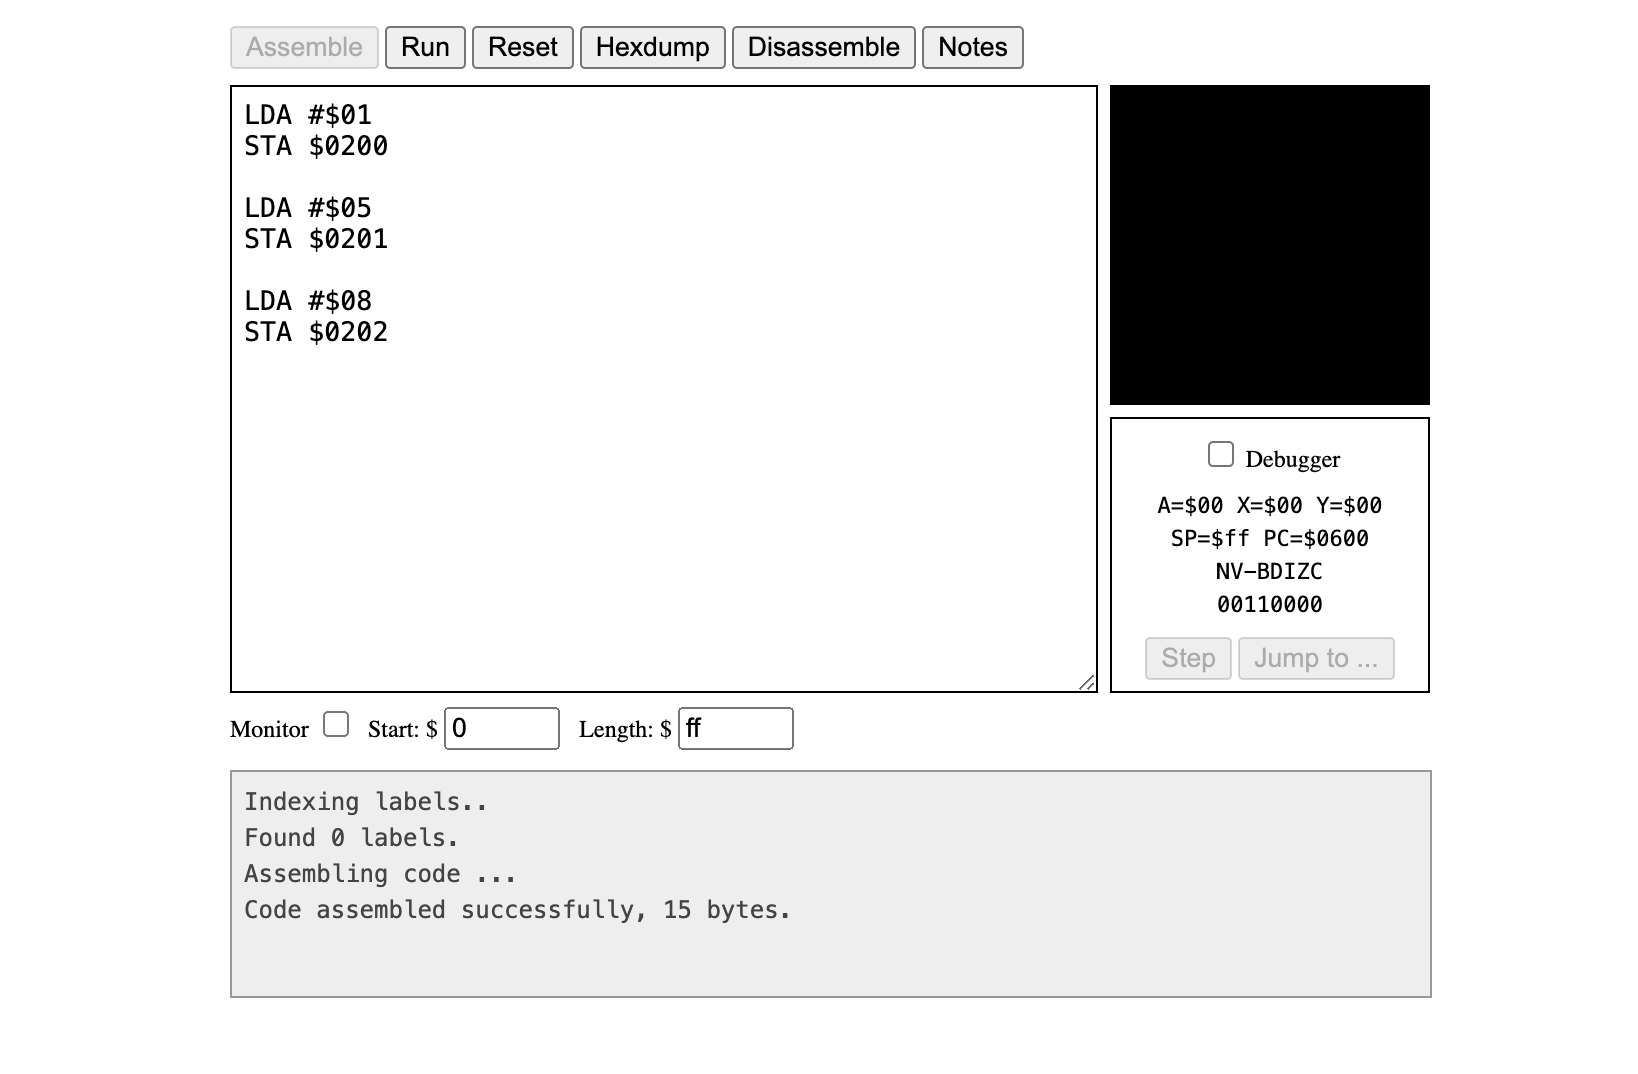
\includegraphics[width=1.0\textwidth]{res/images/q2/01-initial-state.png}
    \caption{Initial state of the 6502 simulator with first program code}
    \label{fig:01-initial-state}
\end{figure}

Now let us see what happened when I ran the code. The result is shown in \textbf{Figure \ref{fig:02-after-running-state}} below. After the simulator is don executing we can see the changes that happened to the $PC$ register. Of course other registers changed, but we will see them later when we try the debugging functionality.

Also the black screen on the top right corner of \textbf{Figure \ref{fig:02-after-running-state}} shows three pixels colored, and that is what the first program instructed the 6502 simulator to do.

\begin{figure}[H]
    \centering
    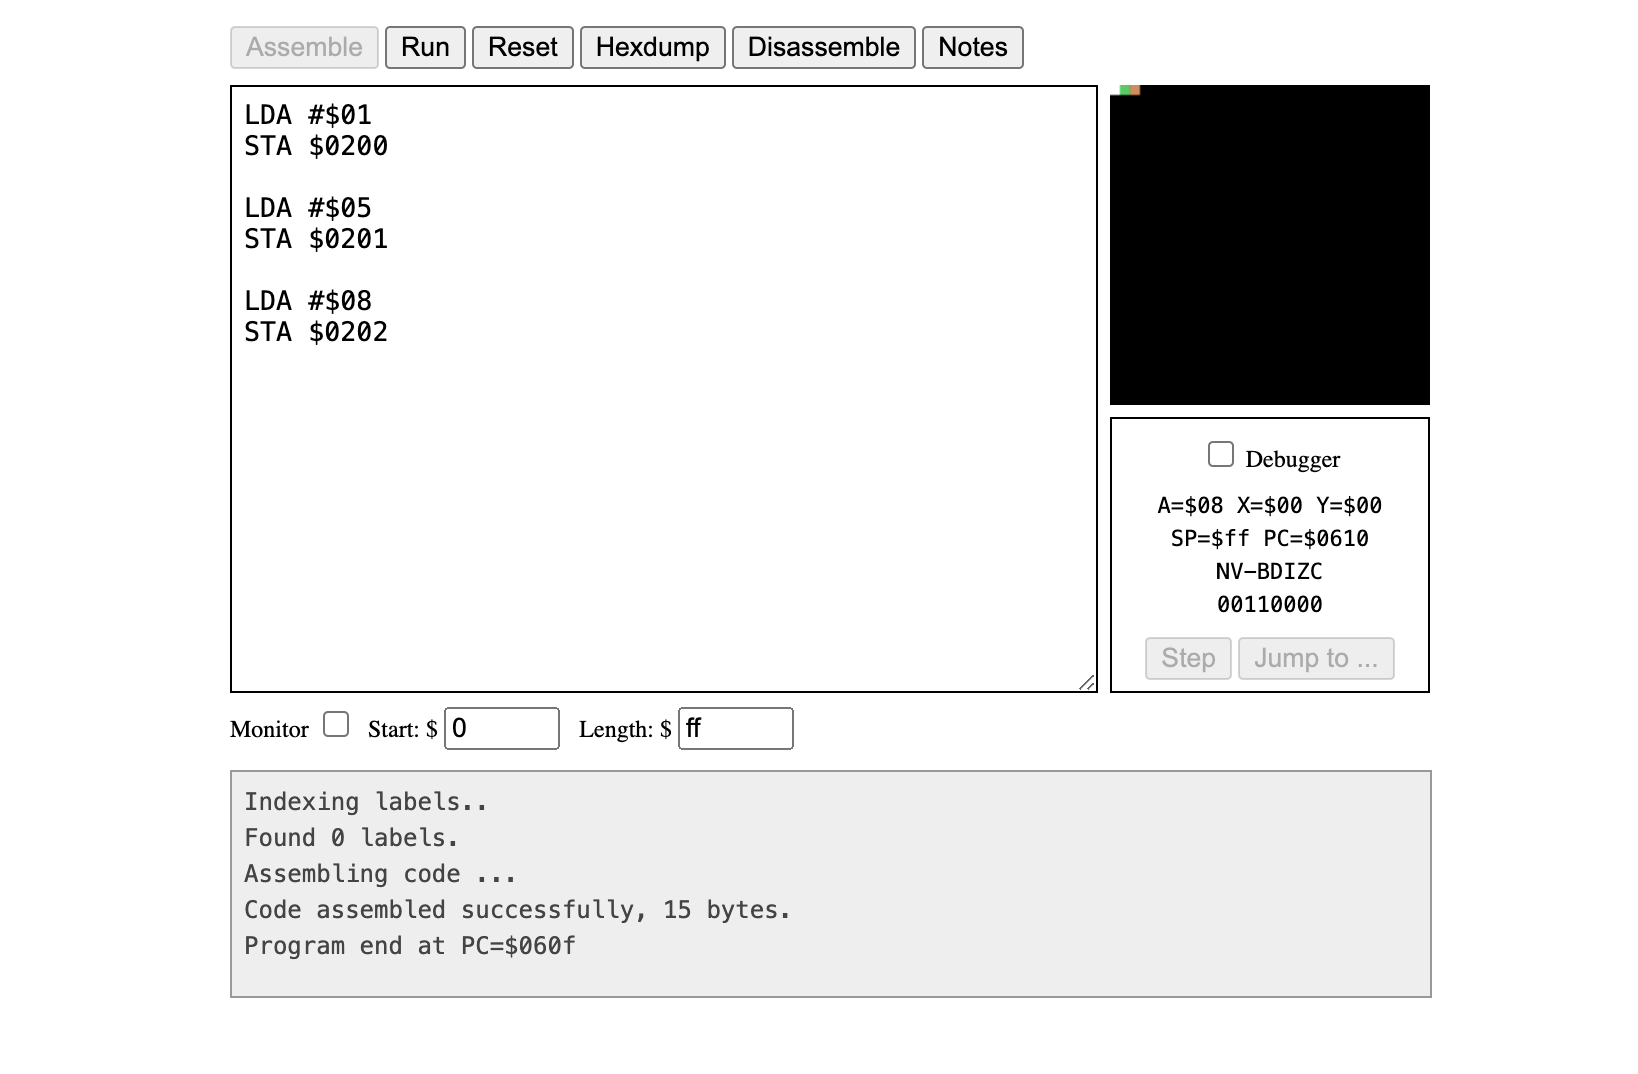
\includegraphics[width=1.0\textwidth]{res/images/q2/02-after-running-state.png}
    \caption{Result of running the first program in the 6502 simulator}
    \label{fig:02-after-running-state}
\end{figure}

Next we will be exploring the debugger functionality in this 6502 simulator. The debugger allows us to step through each CPU cycle manually to allow for debugging, hence the name "debugger". You can use use the debugger by checking the debugger option and then using the step button to step through the assembly code you wrote. You can notice the PC and any other registers you changed, and the memory places for the screen pixels change once you click the step button. I cliked it twice and see what happenned in \textbf{Figure \ref{fig:02-after-running-state}} below. Notice the values of the $A$, the accumulator and $PC$, the program counter, registers.

\begin{figure}[H]
    \centering
    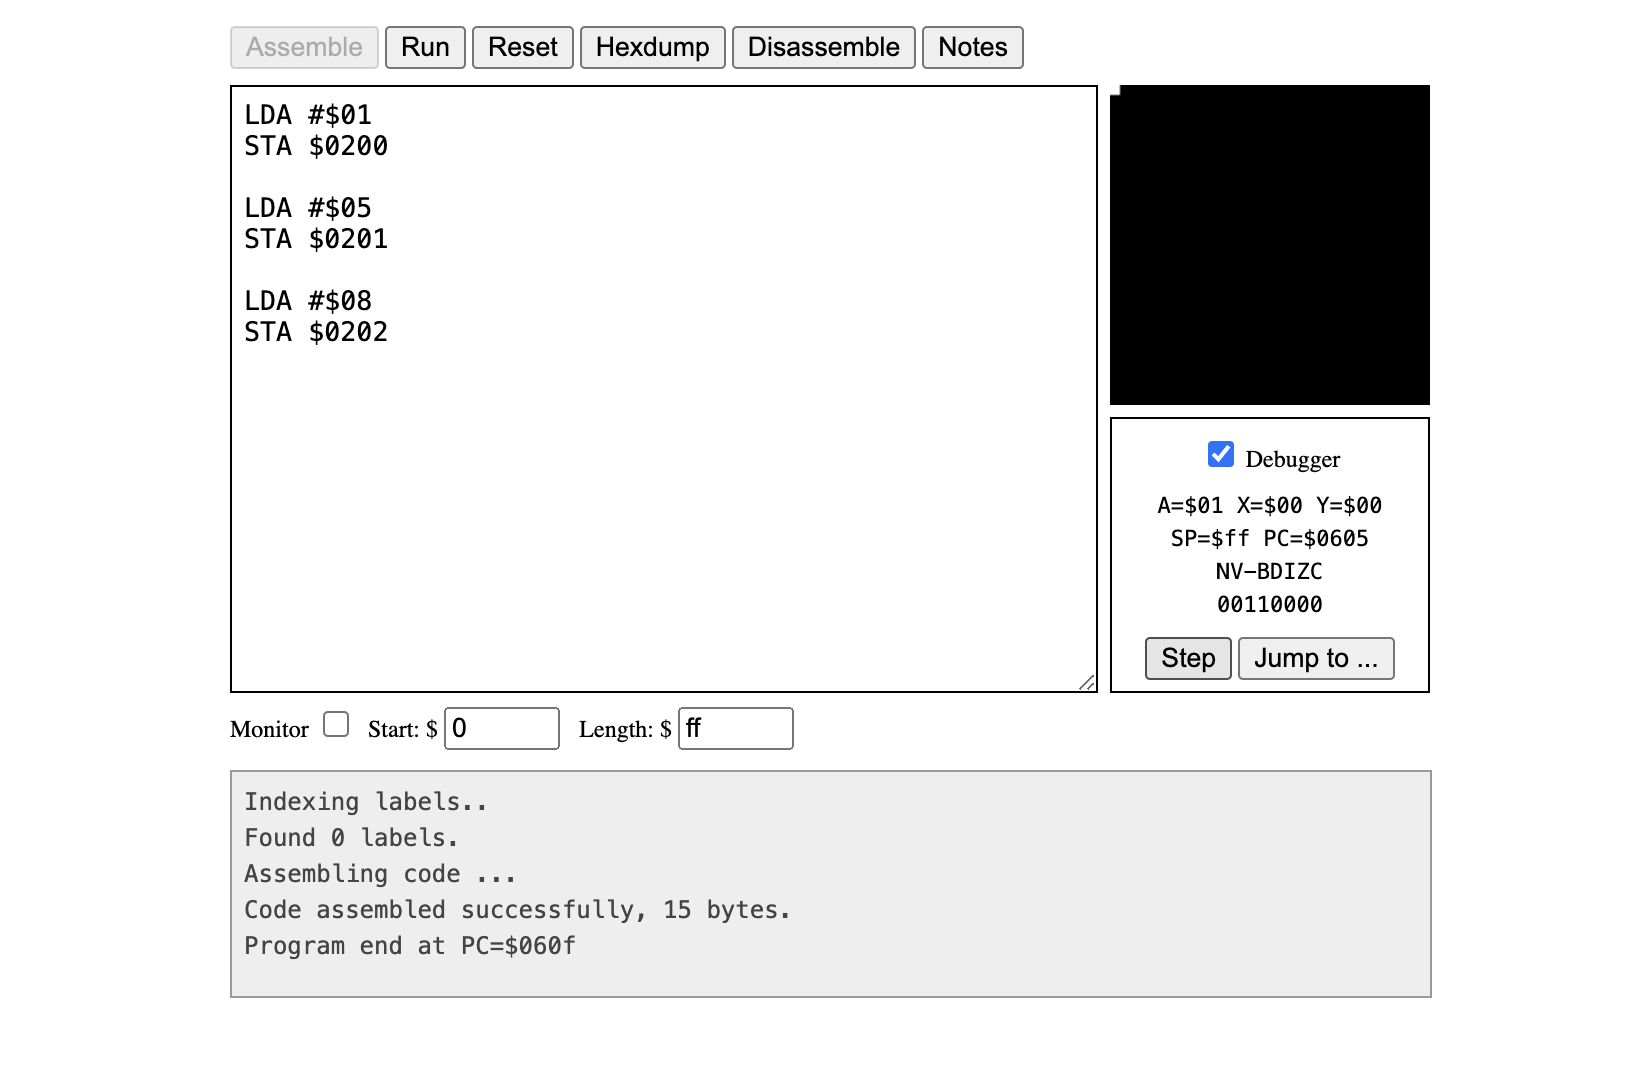
\includegraphics[width=1.0\textwidth]{res/images/q2/03-debugger-first-step.png}
    \caption{Result of running the first program with debugger in the 6502 simulator}
    \label{fig:03-debugger-first-step}
\end{figure}

After this initial trial with the simulator, I will be doing the following exercises and sharing the results below:
\begin{enumerate}
    \item Try changing the colour of the three pixels.
    \item Change one of the pixels to draw at the bottom-right corner (memory location \$05ff).
    \item Add more instructions to draw extra pixels.
\end{enumerate}

\subsubsection{Exercise 1}

I will be editing the code to change the colors, so now the pixels will be showing the following colors in order from left to right: orange, light green, and light blue.

\begin{lstlisting}[style=6502asm]
LDA #$08
STA $0200

LDA #$0d
STA $0201

LDA #$0e
STA $0202
\end{lstlisting}

After the running the code above, the result I got is shown in \textbf{Figure \ref{fig:04-exercise-1}}.

\begin{figure}[H]
    \centering
    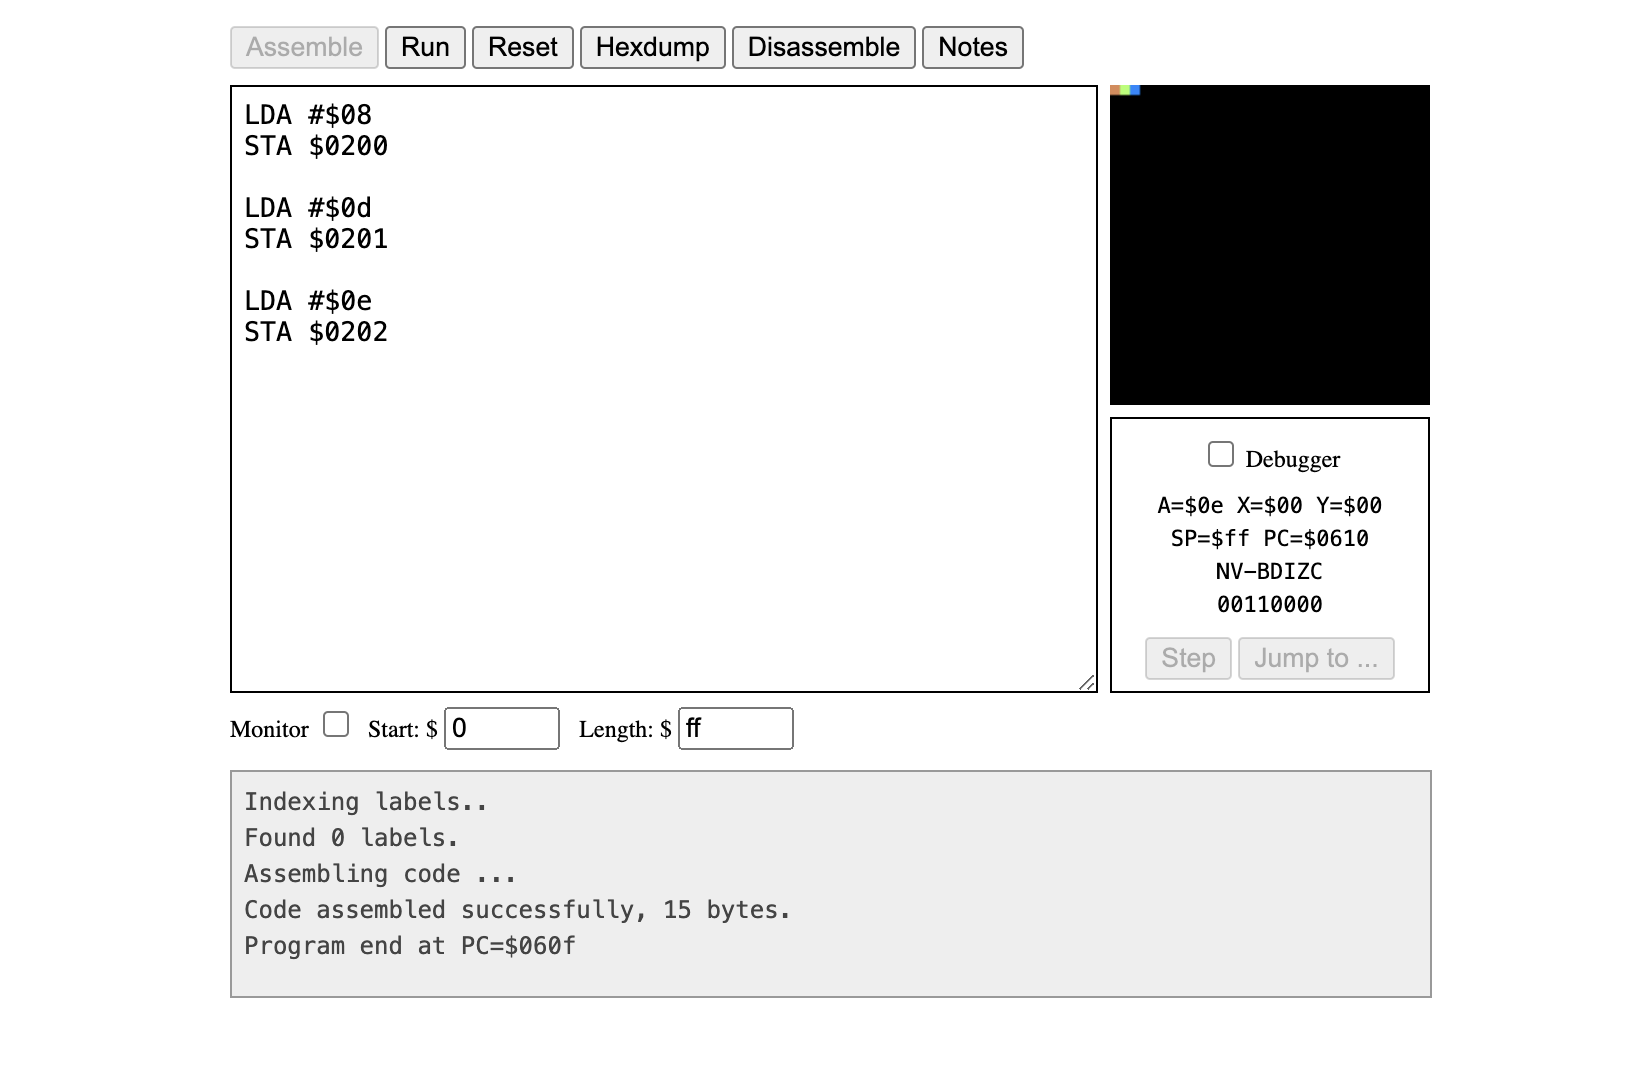
\includegraphics[width=1.0\textwidth]{res/images/q2/04-exercise-1.png}
    \caption{Result of running the first excercise in the 6502 simulator}
    \label{fig:04-exercise-1}
\end{figure}

\subsubsection{Exercise 2}

I will be editing the code from excercise 1 to make the green pixel that was in the middle of the three pixels we rendered before render at the bottom right of the screen. The memory address for that last pixel in the bottom right of the screen is $\$05ff$

\begin{lstlisting}[style=6502asm]
LDA #$08
STA $0200

LDA #$0d
STA $05ff

LDA #$0e
STA $0202
\end{lstlisting}

After the running the code above, the result I got is shown in \textbf{Figure \ref{fig:05-exercise-2}}.

\begin{figure}[H]
    \centering
    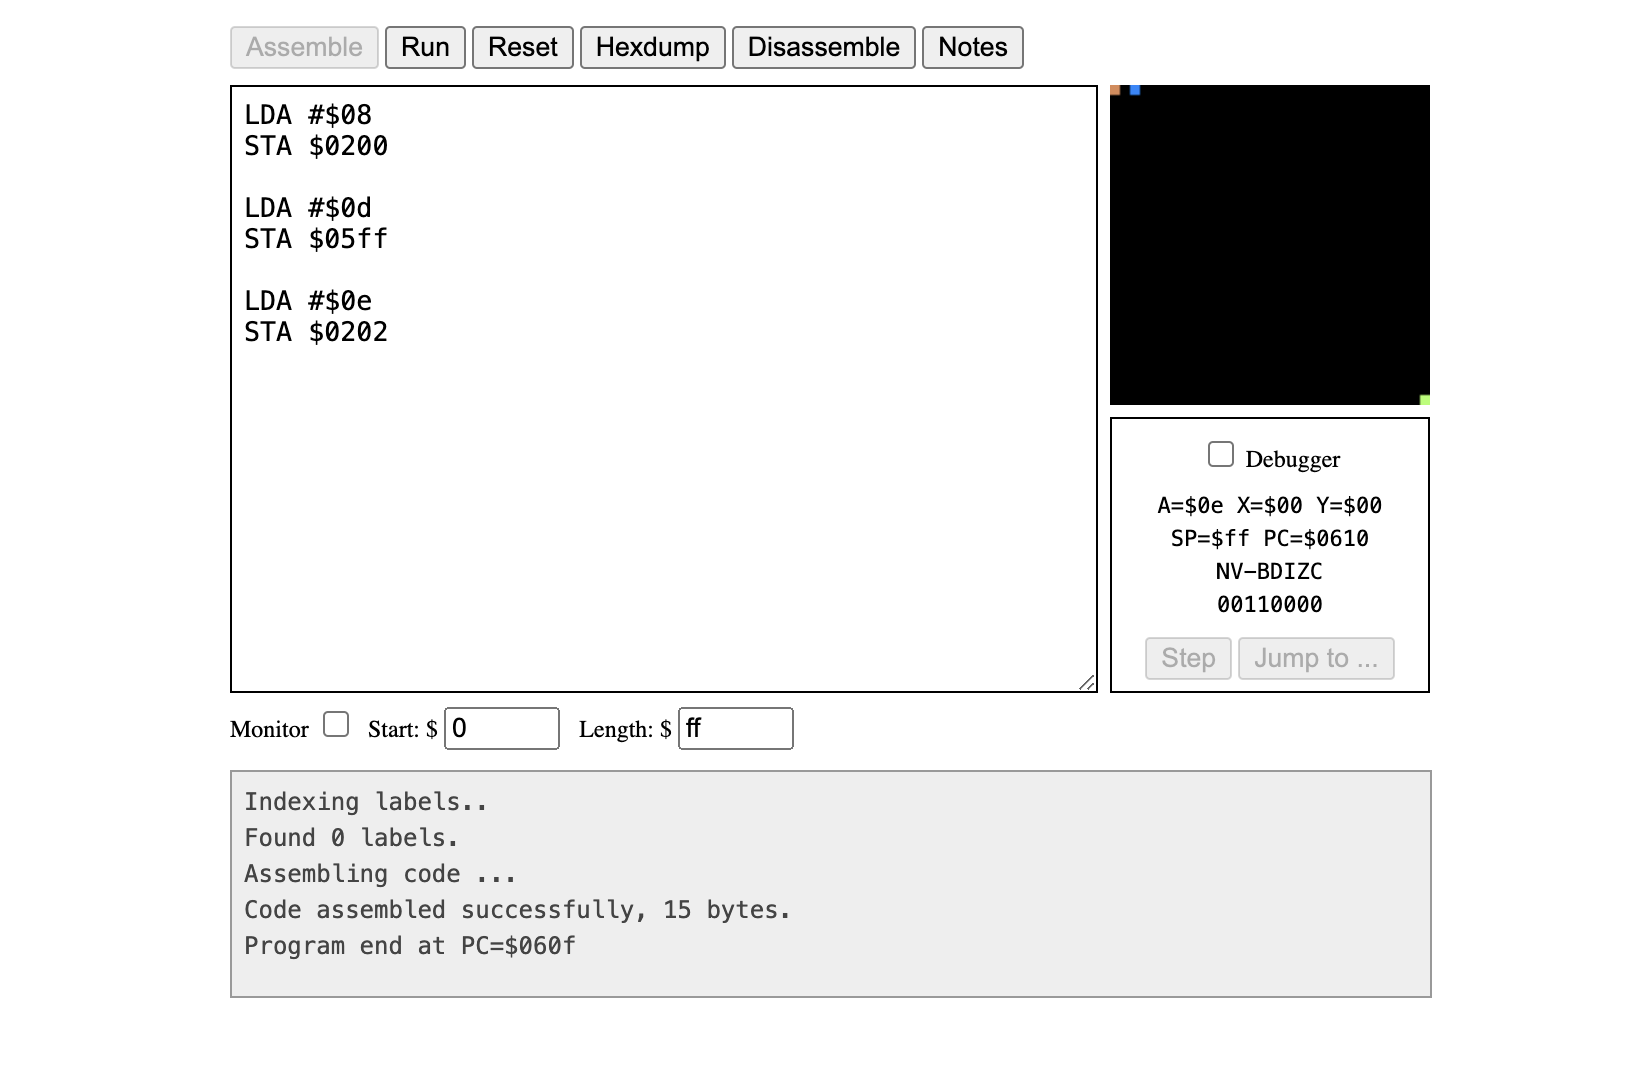
\includegraphics[width=1.0\textwidth]{res/images/q2/05-exercise-2.png}
    \caption{Result of running the second excercise in the 6502 simulator}
    \label{fig:05-exercise-2}
\end{figure}

\subsubsection{Exercise 3}

After the first two exercises, I will be playing more with the pixels and changing the colors. I added pixels in the middle of the screen horizontally spaced equally. The color is both light red and white.

\begin{lstlisting}[style=6502asm]
LDA #$08
STA $0200

LDA #$0d
STA $05ff

LDA #$0e
STA $0202

LDA #$0a
STA $0400
STA $0409

LDX #$01
STX $0410 

STA $0417
STA $041f
\end{lstlisting}

The result is shown in  \textbf{Figure \ref{fig:06-exercise-3}}.

\begin{figure}[H]
    \centering
    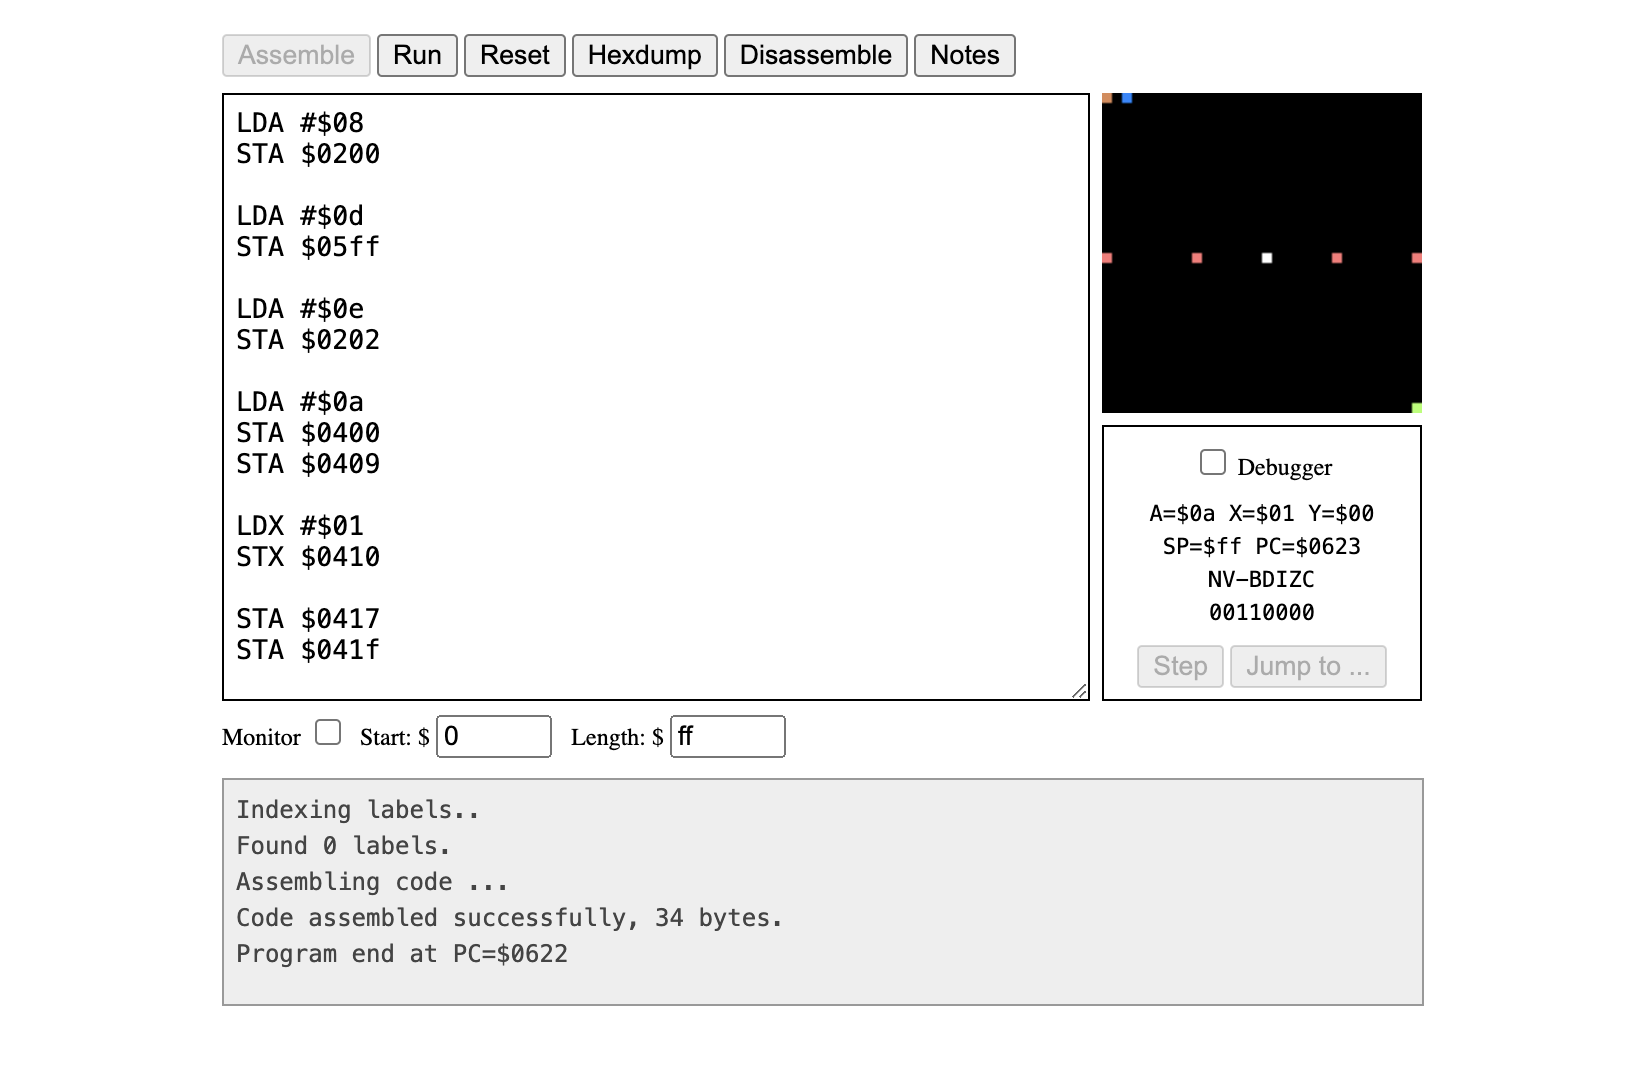
\includegraphics[width=1.0\textwidth]{res/images/q2/06-exercise-3.png}
    \caption{Result of running the third excercise in the 6502 simulator}
    \label{fig:06-exercise-3}
\end{figure}

\subsection{Registers and flags}

Here we learn about the registers and the flags of the CPU. Those can be seen in the simulator in the "processor status" section, shown in  \textbf{Figure \ref{fig:07-register-and-flags}}. The registers this 6502 simulator has are:

\begin{itemize}
    \item $A$ register: the accumulator, holds a single byte.
    \item $X$ register: a generic register, holds a single byte.
    \item $Y$ register: another generic register, holds a single byte.
    \item $SP$ register: stack pointer, basically this register is decremented every time a byte is pushed onto the stack, and decremented when a byte is popped off the stack.
    \item $PC$ register: program counter, tells the CPU where the program is currently at in the memory, it is incremented every CPU cycle unless some $JMP$ happens or something that interrupts the CPU.
\end{itemize}

\begin{figure}[H]
    \centering
    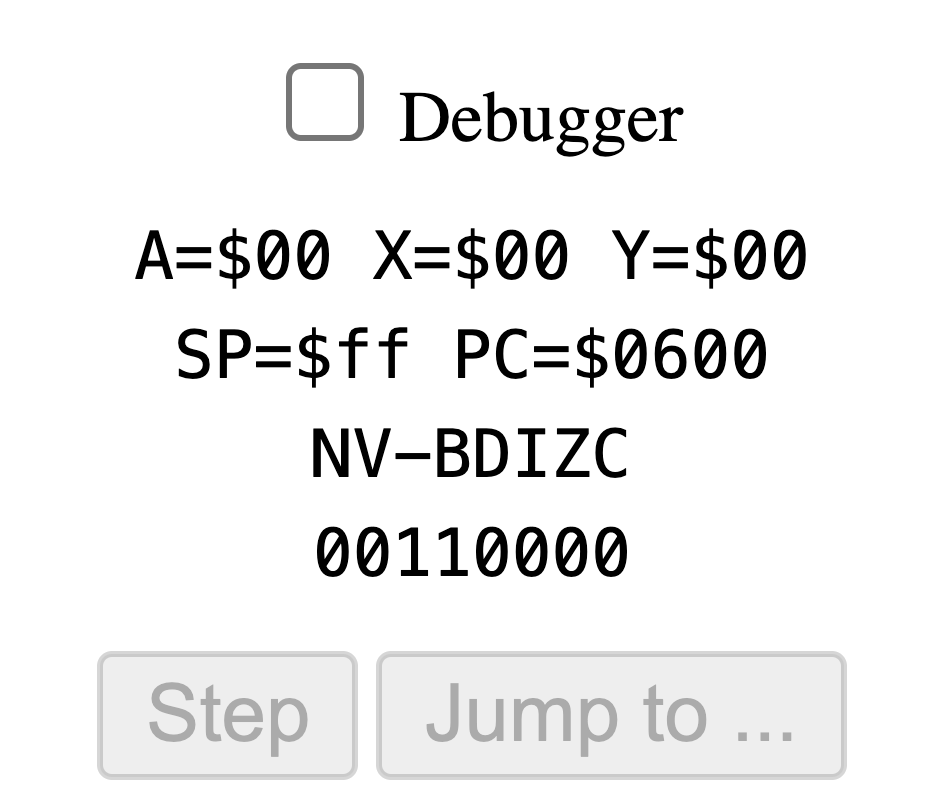
\includegraphics[width=0.5\textwidth]{res/images/q2/07-register-and-flags.png}
    \caption{Processor status section in the 6502 simulator}
    \label{fig:07-register-and-flags}
\end{figure}

Enough about the top section of the processor status section, let us talk about the bottom section that contains the processor flags. Each flag is one bit, so the seven flags we have can be represented as one byte. The flags are set byt the processor to give information about the previous instruction.

\subsection{Instructions}

Instructions in the 6502 assembly language are 56, we will be exploring some of them.

\subsubsection{First Program}

The first piece of code we have is the following:

\begin{lstlisting}[style=6502asm]
LDA #$c0  ;Load the hex value $c0 into the A register
TAX       ;Transfer the value in the A register to X
INX       ;Increment the value in the X register
ADC #$c4  ;Add the hex value $c4 to the A register
BRK       ;Break - we're done
\end{lstlisting}

Now let us use the debugger to step through this code above. \textbf{Figure \ref{fig:08-instructions-first-initial}} shows the initial state of the simulator.

\begin{figure}[H]
    \centering
    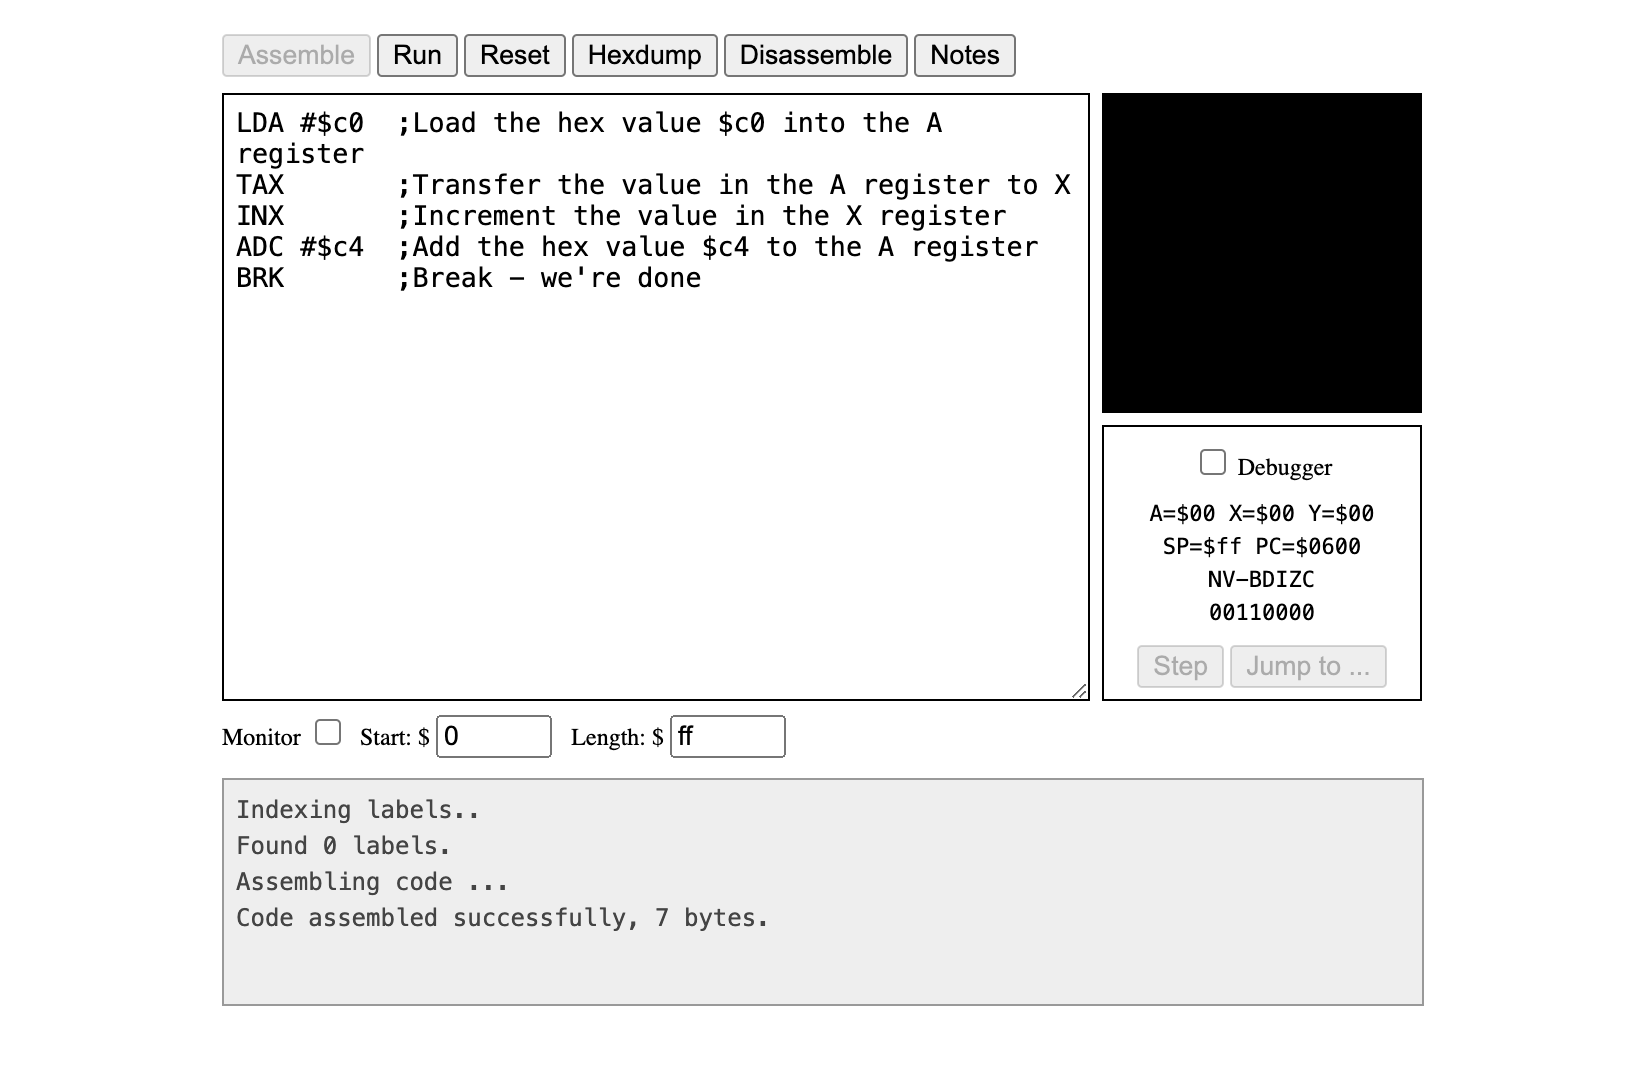
\includegraphics[width=1.0\textwidth]{res/images/q2/08-instructions-first-initial.png}
    \caption{Initial state of first program in instructions in the 6502 simulator}
    \label{fig:08-instructions-first-initial}
\end{figure}

We then step 4 times, let us view them below in order. The figures in order are: \textbf{Figure \ref{fig:09-instructions-first-step1}}, \textbf{Figure \ref{fig:10-instructions-first-step2}}, \textbf{Figure \ref{fig:11-instructions-first-step3}}, and \textbf{Figure \ref{fig:12-instructions-first-step4}}

\begin{figure}[H]
    \centering
    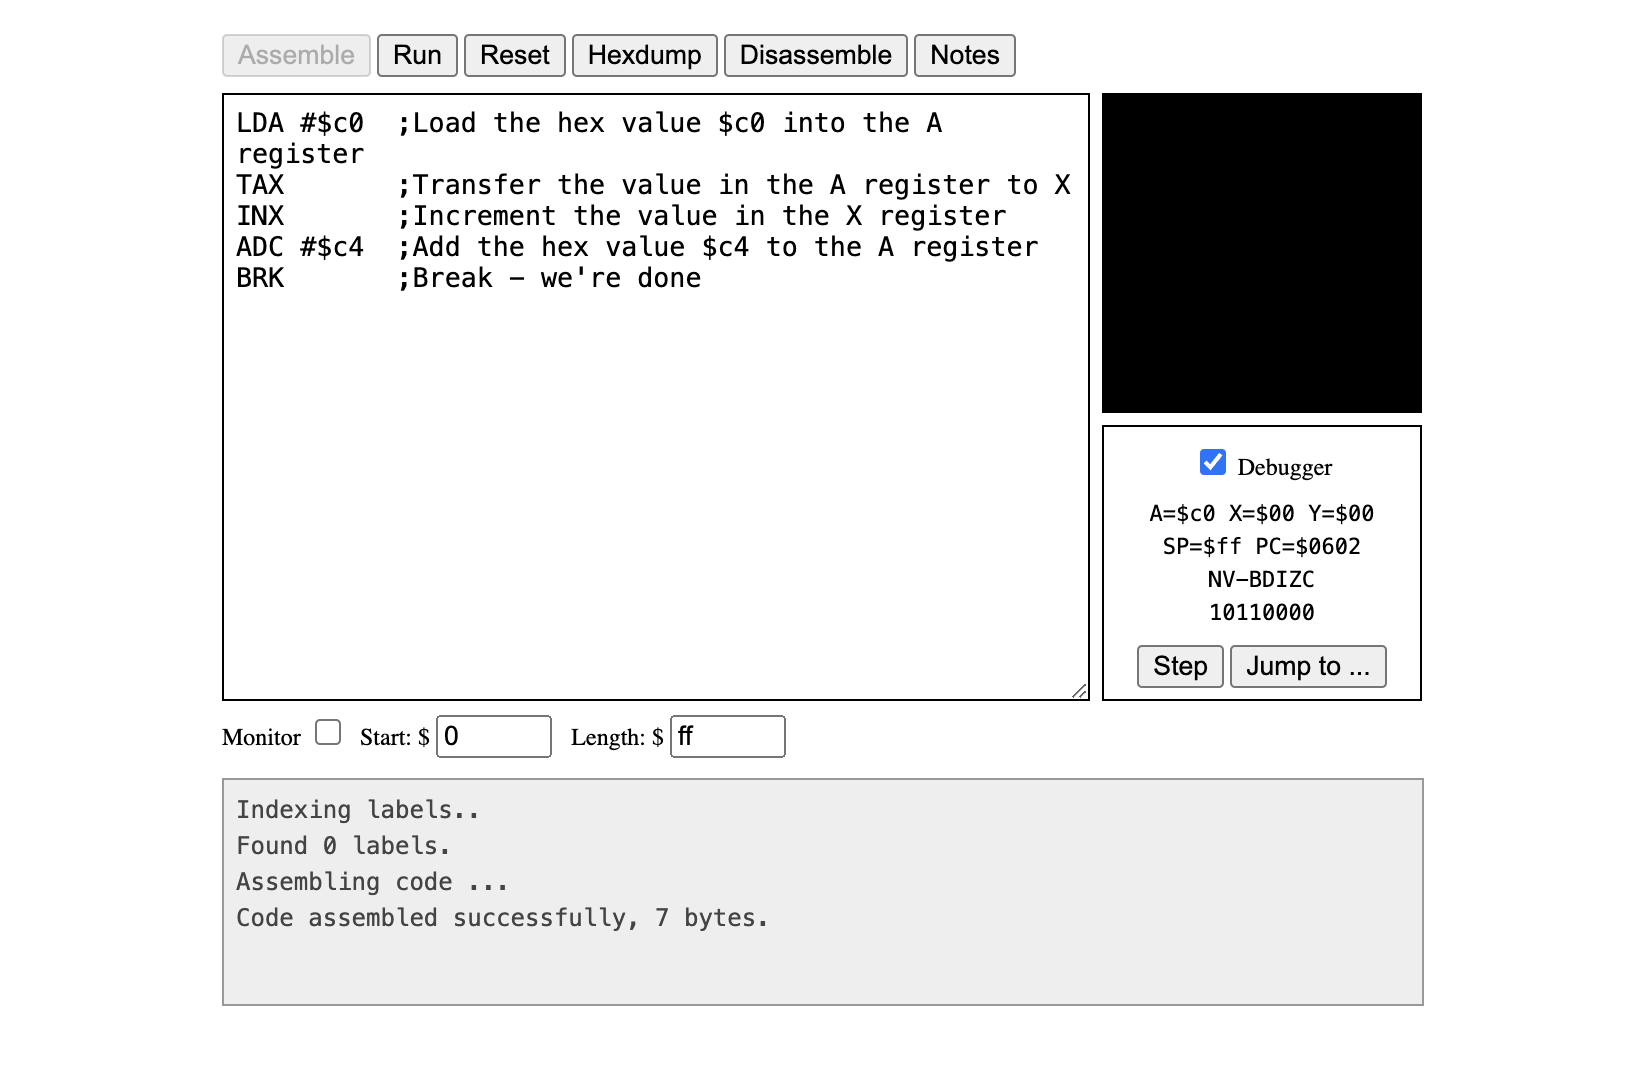
\includegraphics[width=1.0\textwidth]{res/images/q2/09-instructions-first-step1.png}
    \caption{First step of first program in instructions in the 6502 simulator}
    \label{fig:09-instructions-first-step1}
\end{figure}

\begin{figure}[H]
    \centering
    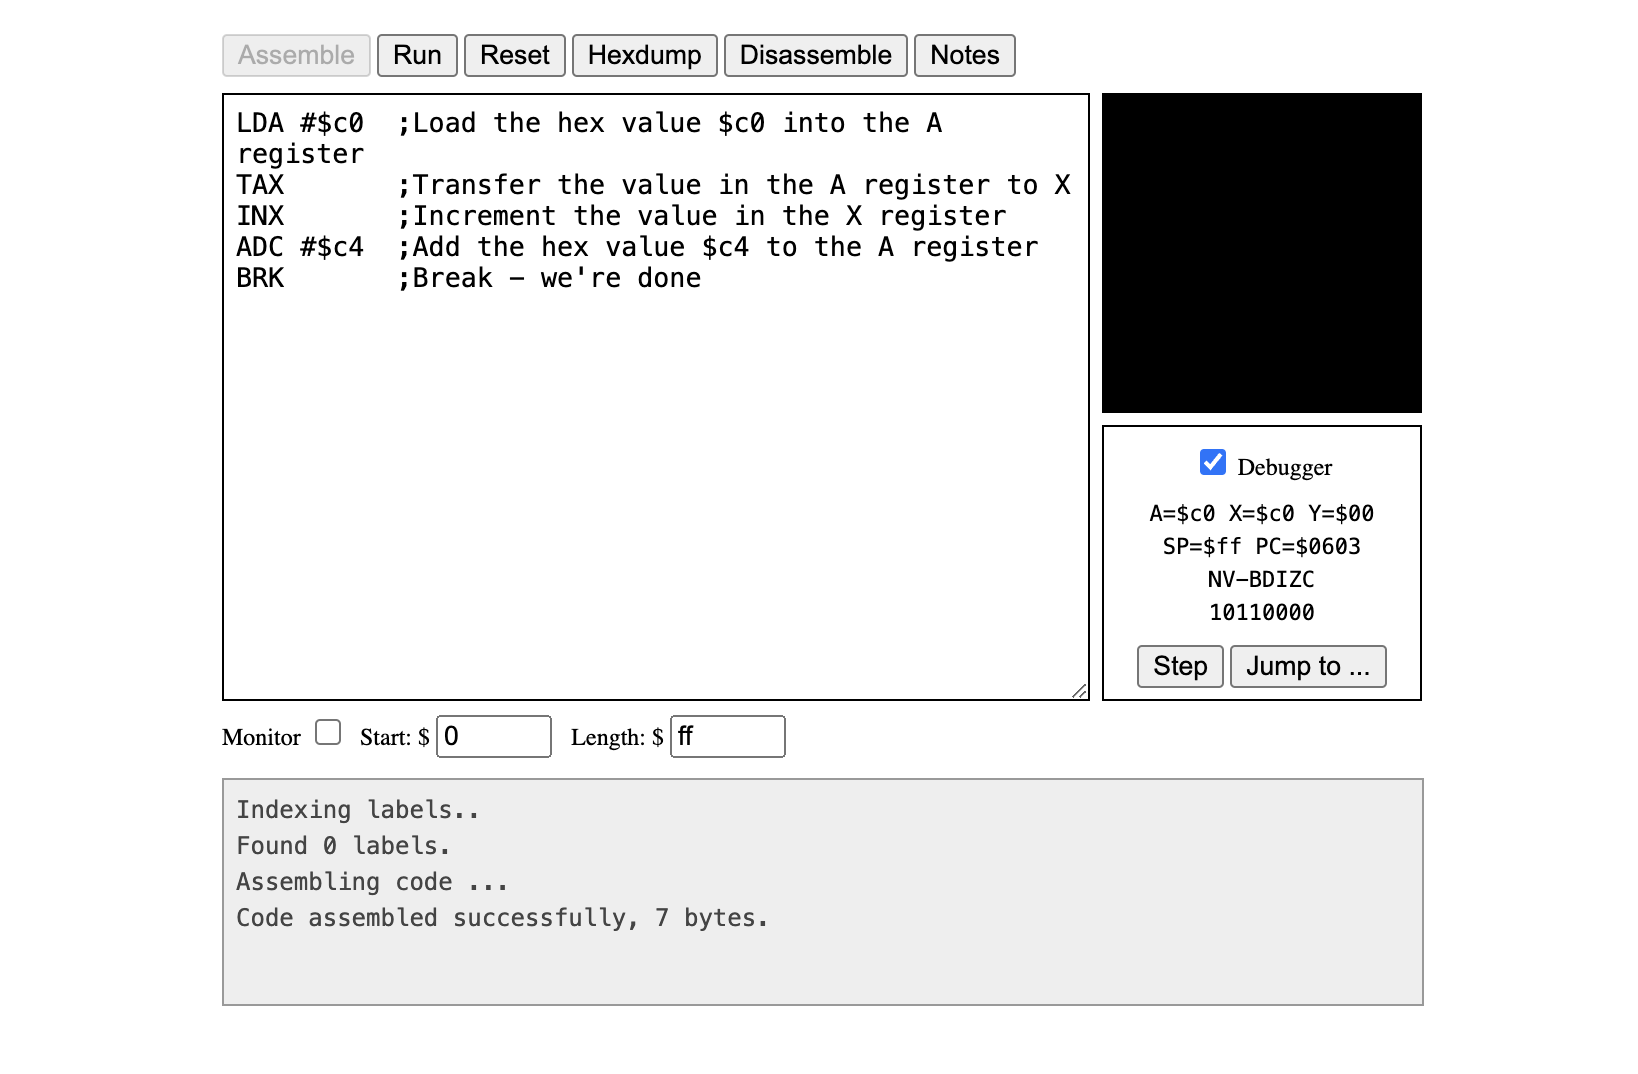
\includegraphics[width=1.0\textwidth]{res/images/q2/10-instructions-first-step2.png}
    \caption{Second step of first program in instructions in the 6502 simulator}
    \label{fig:10-instructions-first-step2}
\end{figure}

\begin{figure}[H]
    \centering
    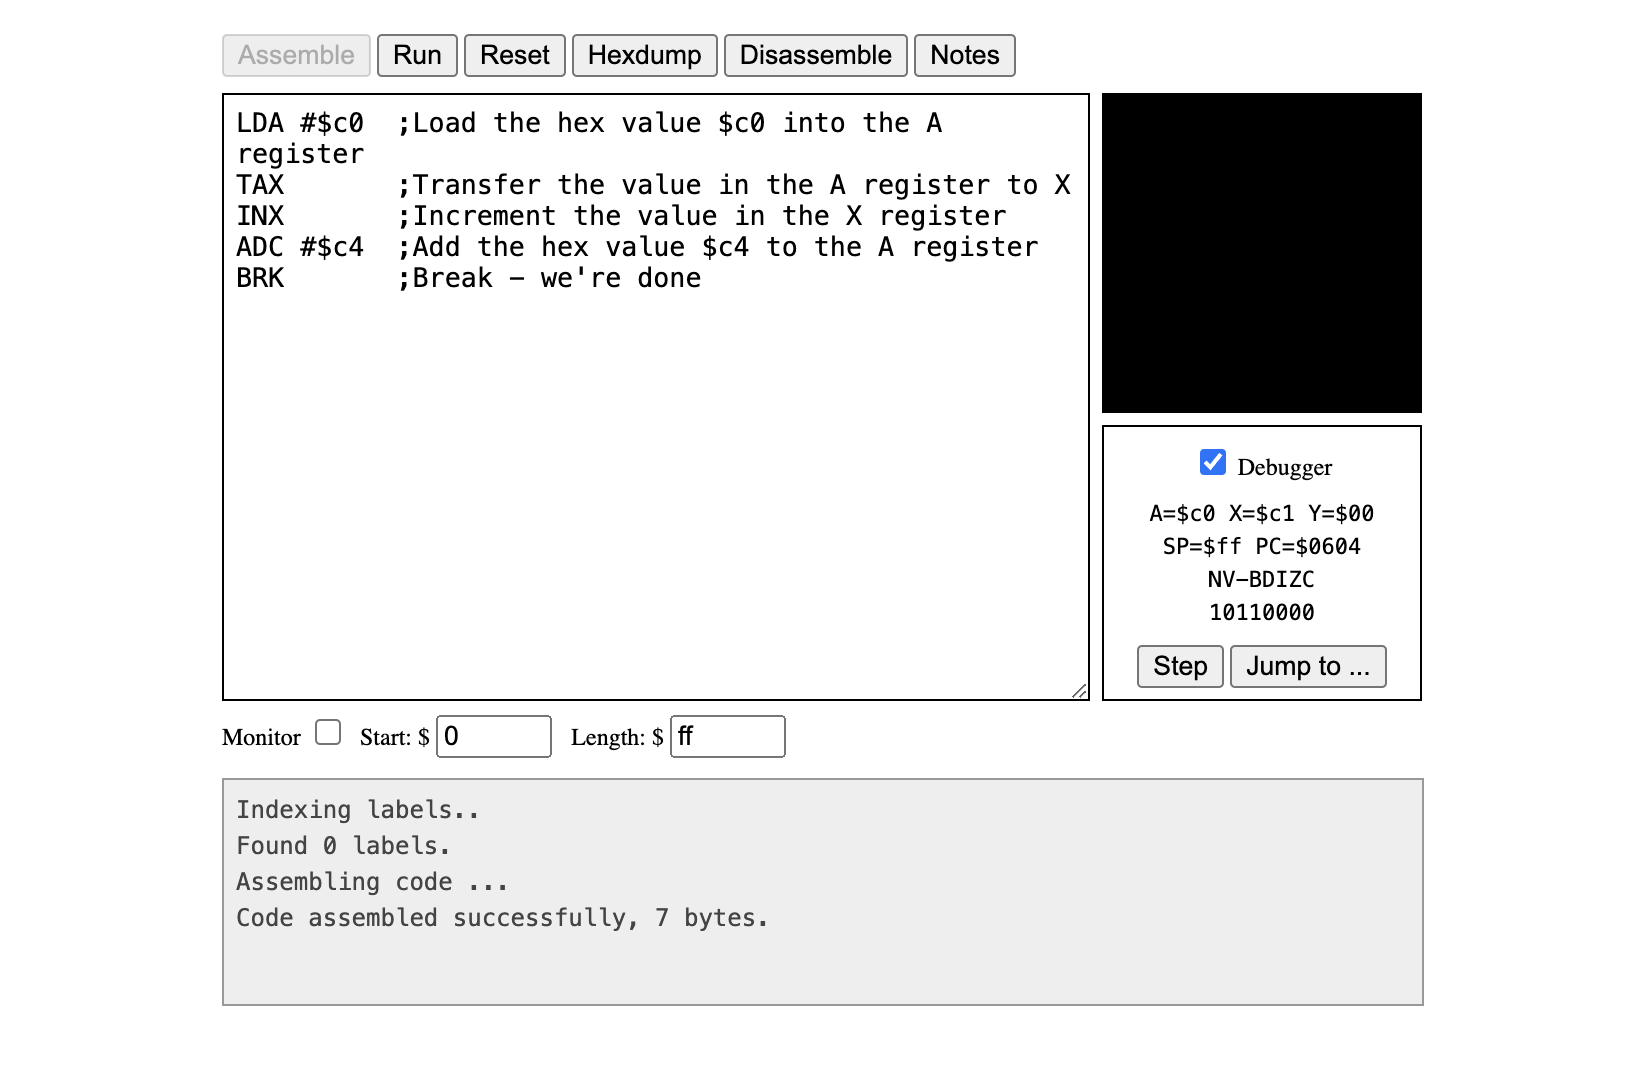
\includegraphics[width=1.0\textwidth]{res/images/q2/11-instructions-first-step3.png}
    \caption{Third step of first program in instructions in the 6502 simulator}
    \label{fig:11-instructions-first-step3}
\end{figure}

\begin{figure}[H]
    \centering
    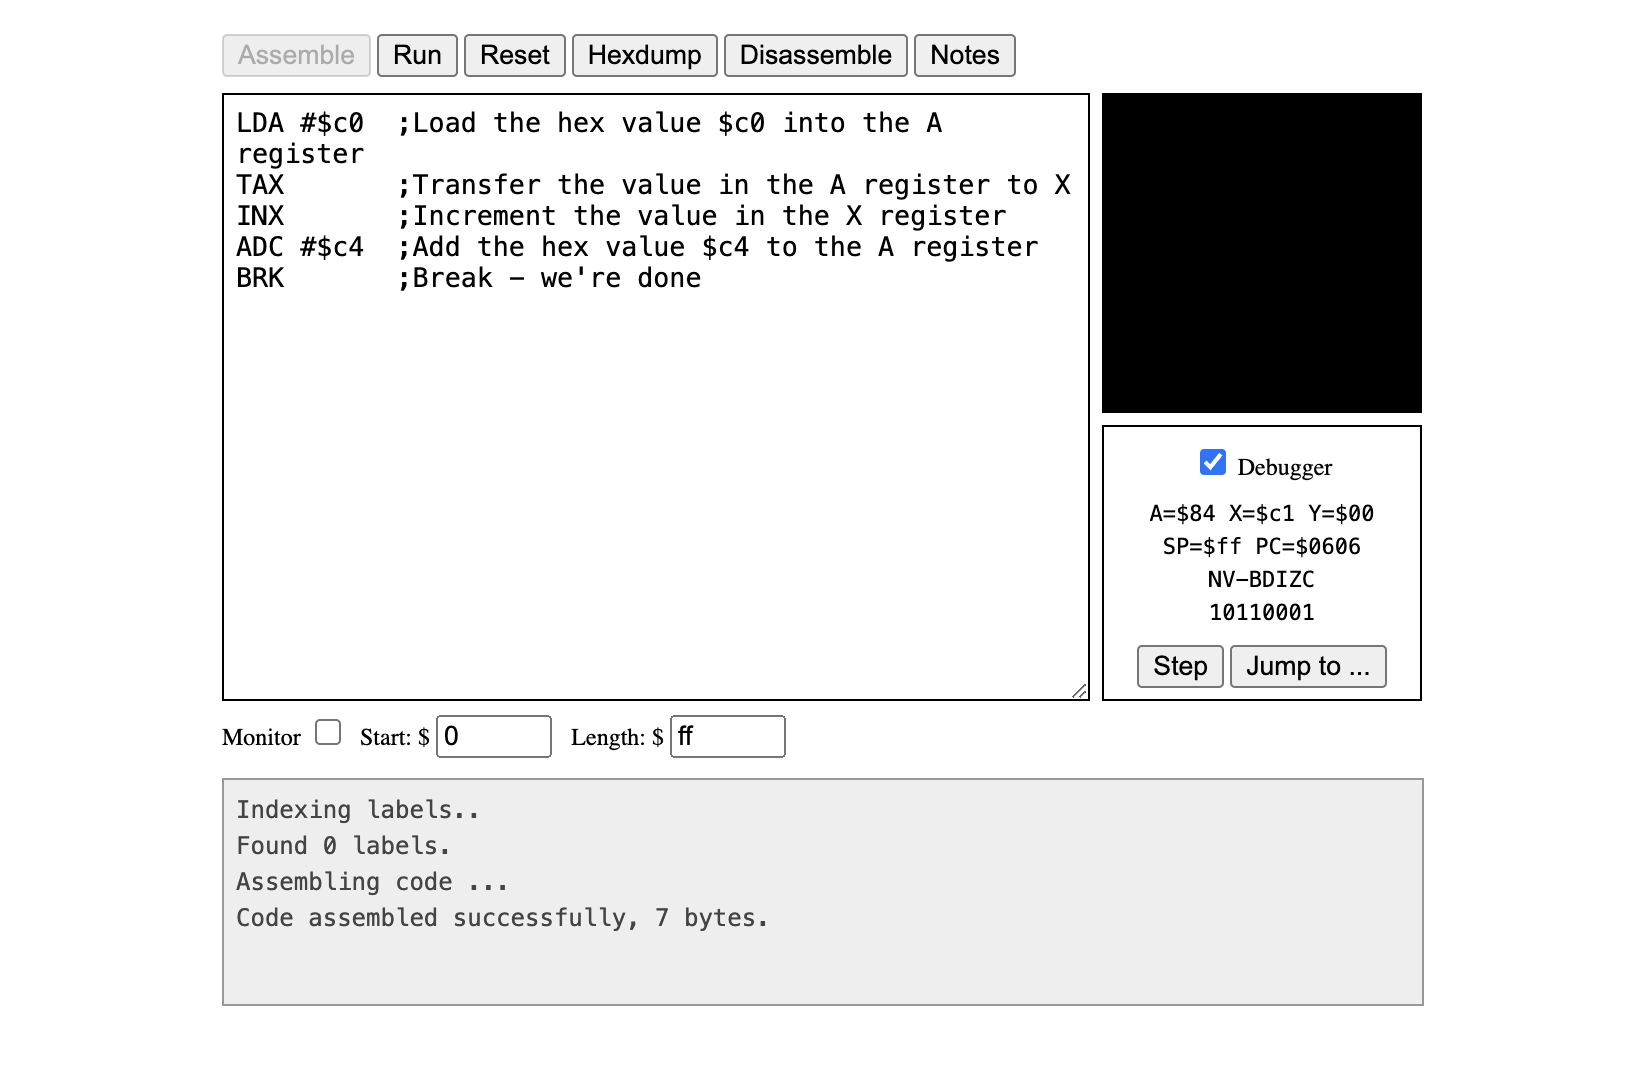
\includegraphics[width=1.0\textwidth]{res/images/q2/12-instructions-first-step4.png}
    \caption{Fourth step of first program in instructions in the 6502 simulator}
    \label{fig:12-instructions-first-step4}
\end{figure}

In the last step, \textbf{Figure \ref{fig:12-instructions-first-step4}}, you might expect that adding $\$c4$ to register $A$ will yield the result $\$184$ but we are getting $\$84$. That is because the maximum number the register can handle is one byte, and $\$184$ is bigger than $\$FF$. And we can also notice that the processor carry flag was set to $1$, and that's how we know that there is something weird. The carry flag is the last bit in the $NV-DBIZC$, hence the $C$.

\subsubsection{Second Program}

The second piece of code in this section is the following:

\begin{lstlisting}[style=6502asm]
LDA #$80
STA $01
ADC $01
\end{lstlisting}

Notice an important thing regarding the $ADC$ opcode, in the first example there was a $\#$ but now there is no $\#$. When we have a leading $\#$, the assembler will regards it as a number. But when it is directly stated like $\$01$, it replaces it with the value stored at that memory location.

Before running this code, we will tick the monitor checkbox so we can see the memory visually:

\begin{figure}[H]
    \centering
    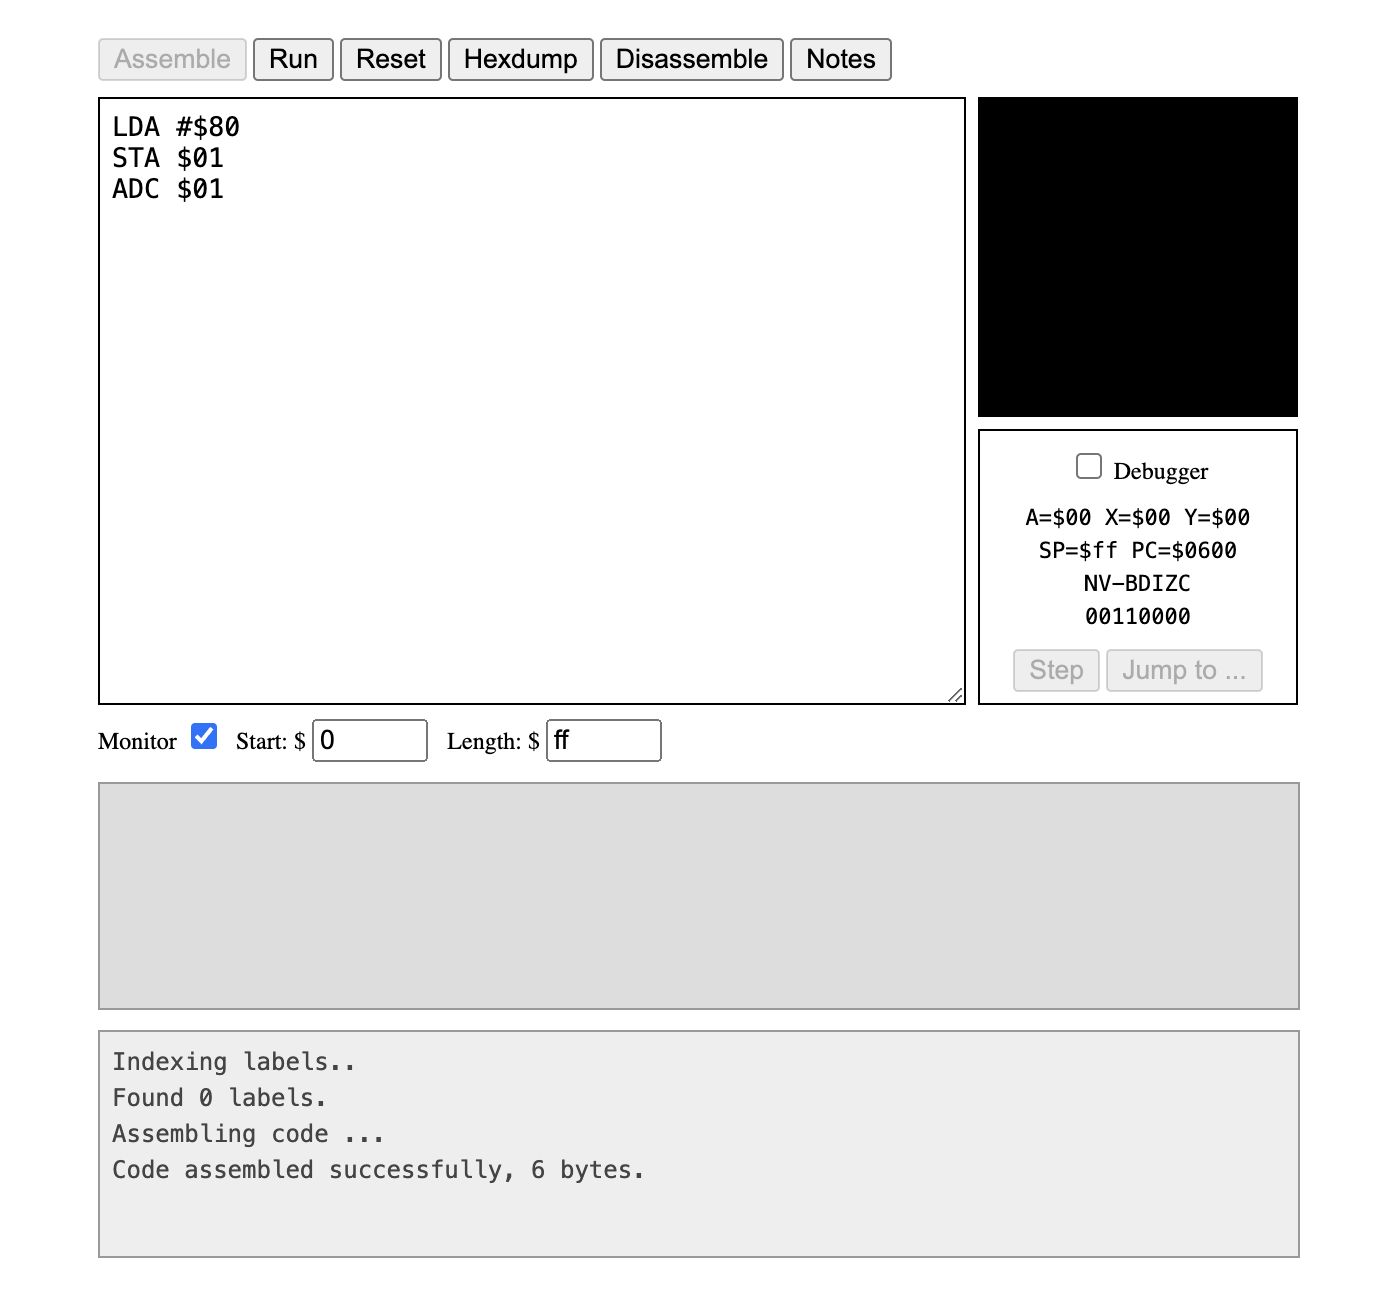
\includegraphics[width=1.0\textwidth]{res/images/q2/13-instructions-second-initial.png}
    \caption{Initial state of second program in instructions in the 6502 simulator}
    \label{fig:13-instructions-second-initial}
\end{figure}

Now we will be stepping through the code, three steps since they are three lines. Let us look at what happens to the memory in \textbf{Figure \ref{fig:15-instructions-second-step2}}.

\begin{figure}[H]
    \centering
    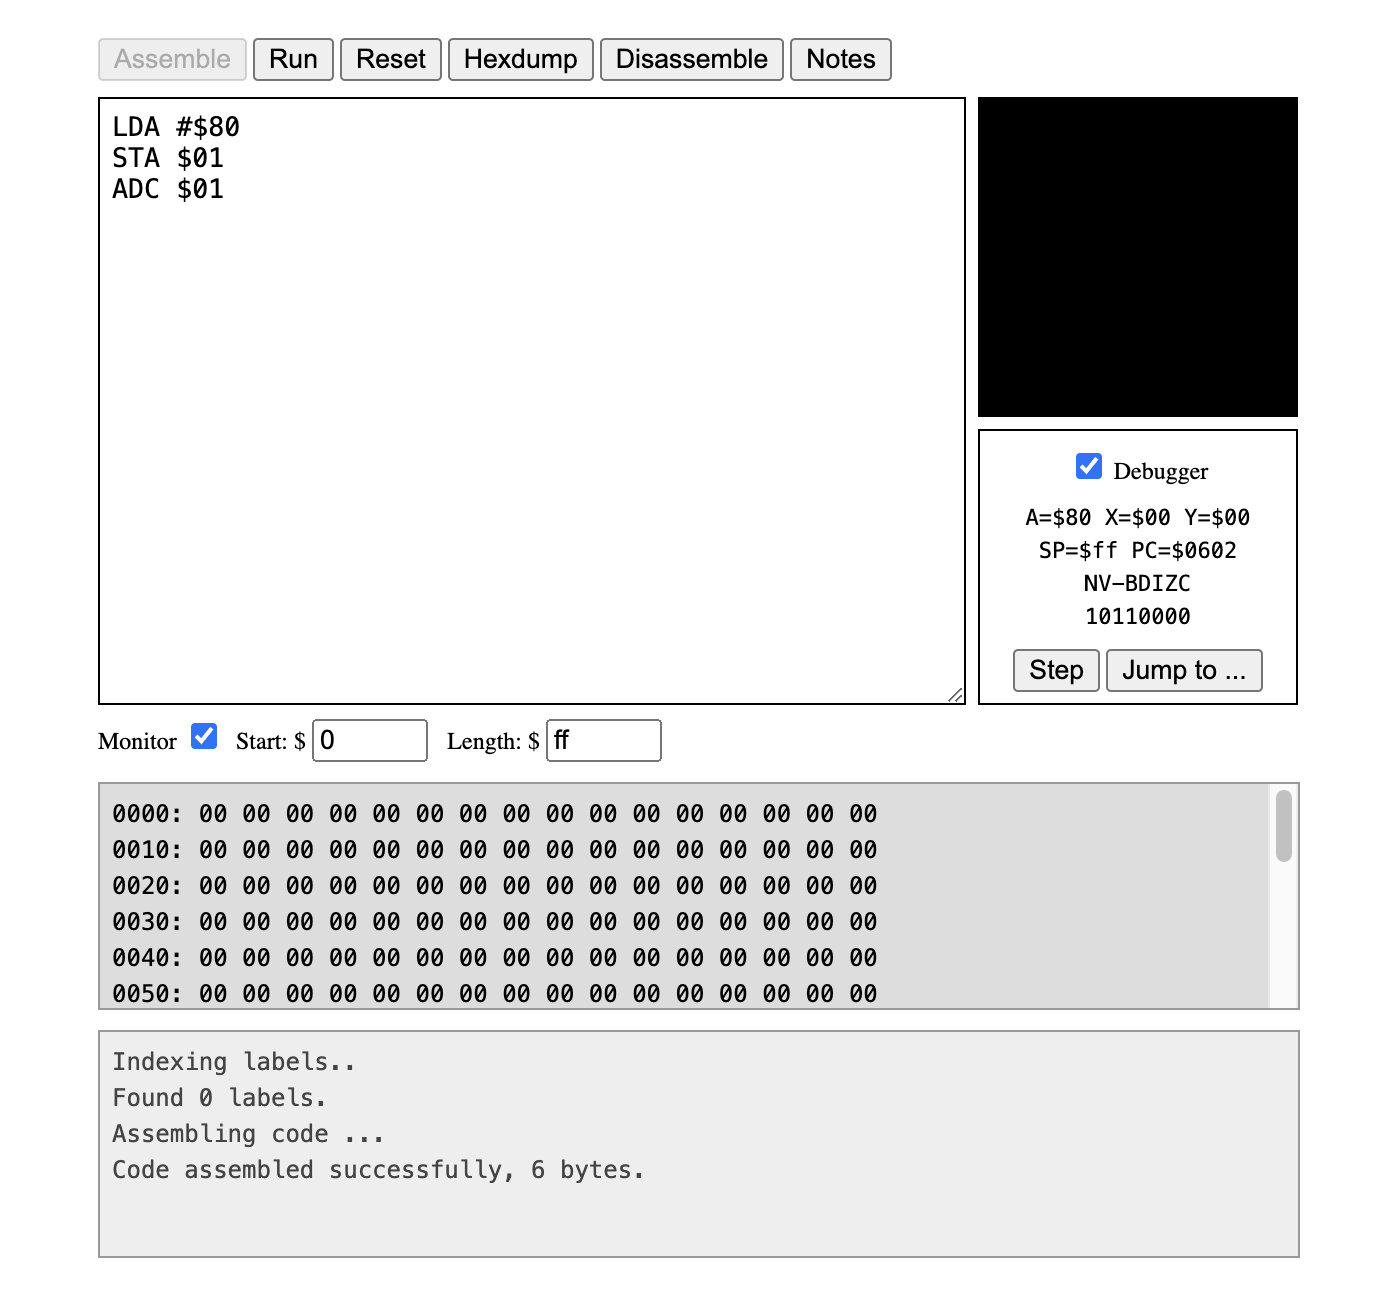
\includegraphics[width=1.0\textwidth]{res/images/q2/14-instructions-second-step1.png}
    \caption{Step 1 of second program in instructions in the 6502 simulator}
    \label{fig:14-instructions-second-step1}
\end{figure}

In \textbf{Figure \ref{fig:14-instructions-second-step1}}, the number 80 is loaded into register $A$. Notice how the memory is made up of ZEROs, that means it is empty for now.

\begin{figure}[H]
    \centering
    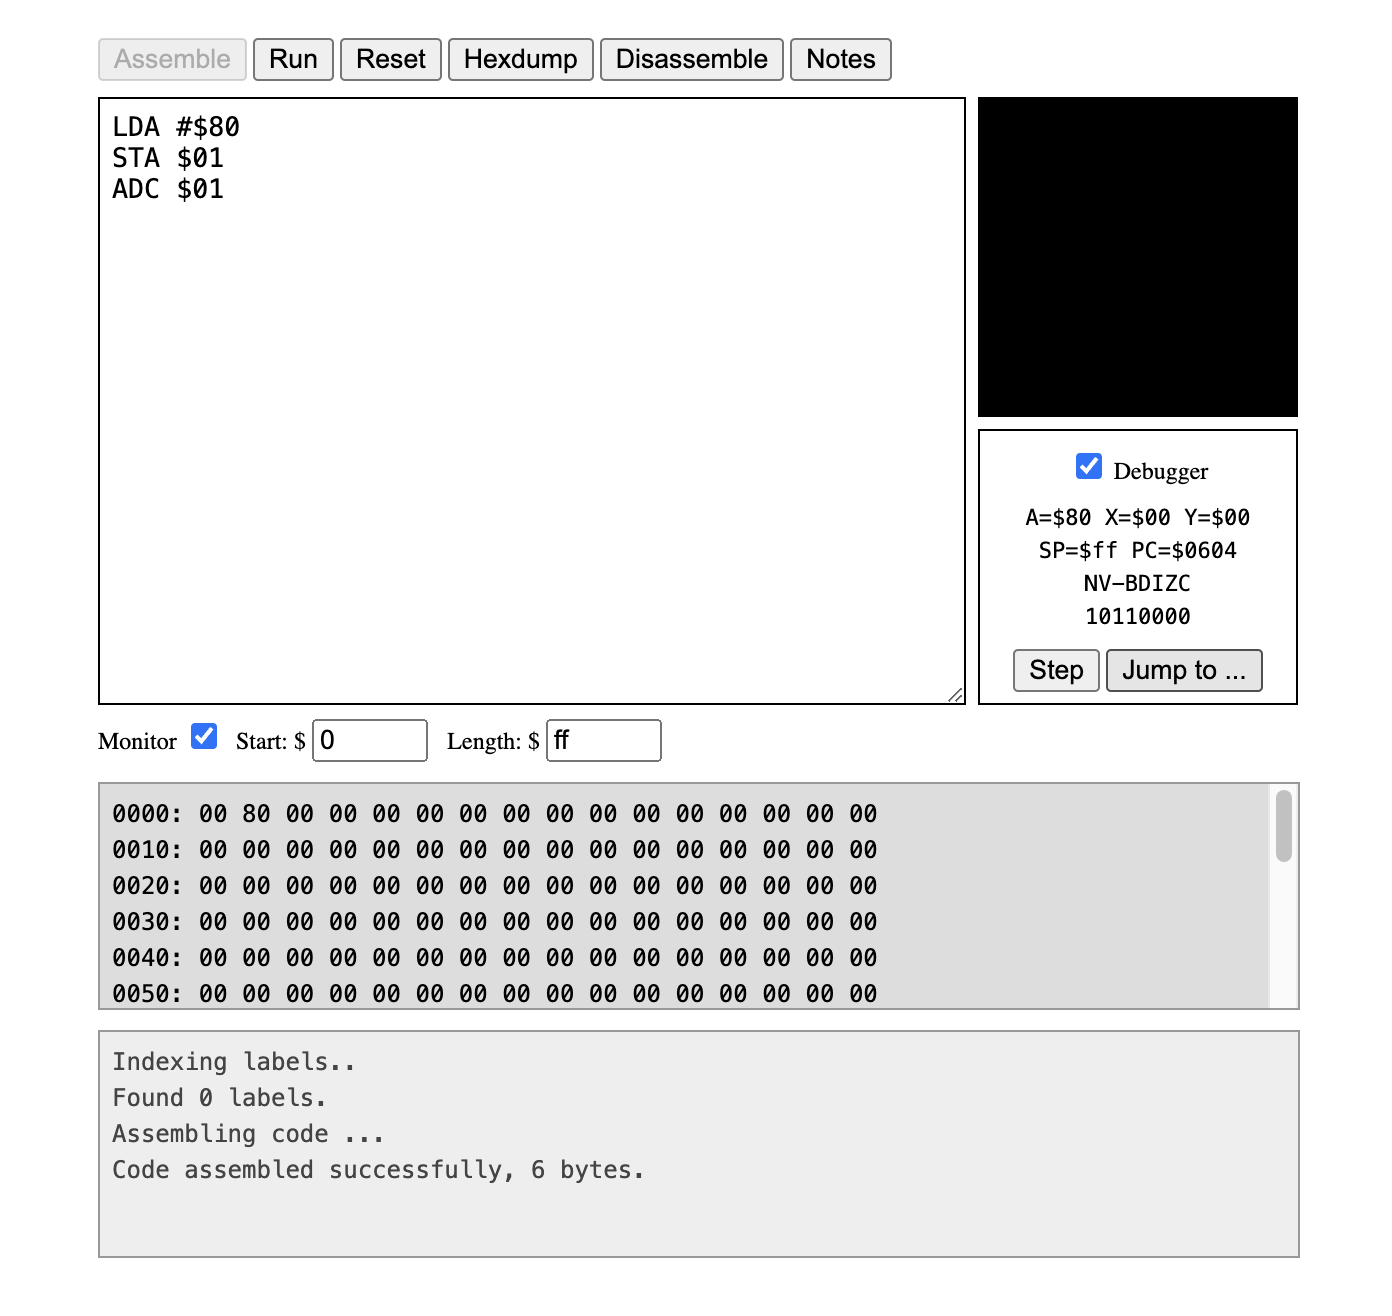
\includegraphics[width=1.0\textwidth]{res/images/q2/15-instructions-second-step2.png}
    \caption{Step 2 of second program in instructions in the 6502 simulator}
    \label{fig:15-instructions-second-step2}
\end{figure}

After that in \textbf{Figure \ref{fig:15-instructions-second-step2}}, the value held in register $A$, aka the accumulator, is saved at the memory location $\$01$. You can notice it in the monitor in the first line.

\begin{figure}[H]
    \centering
    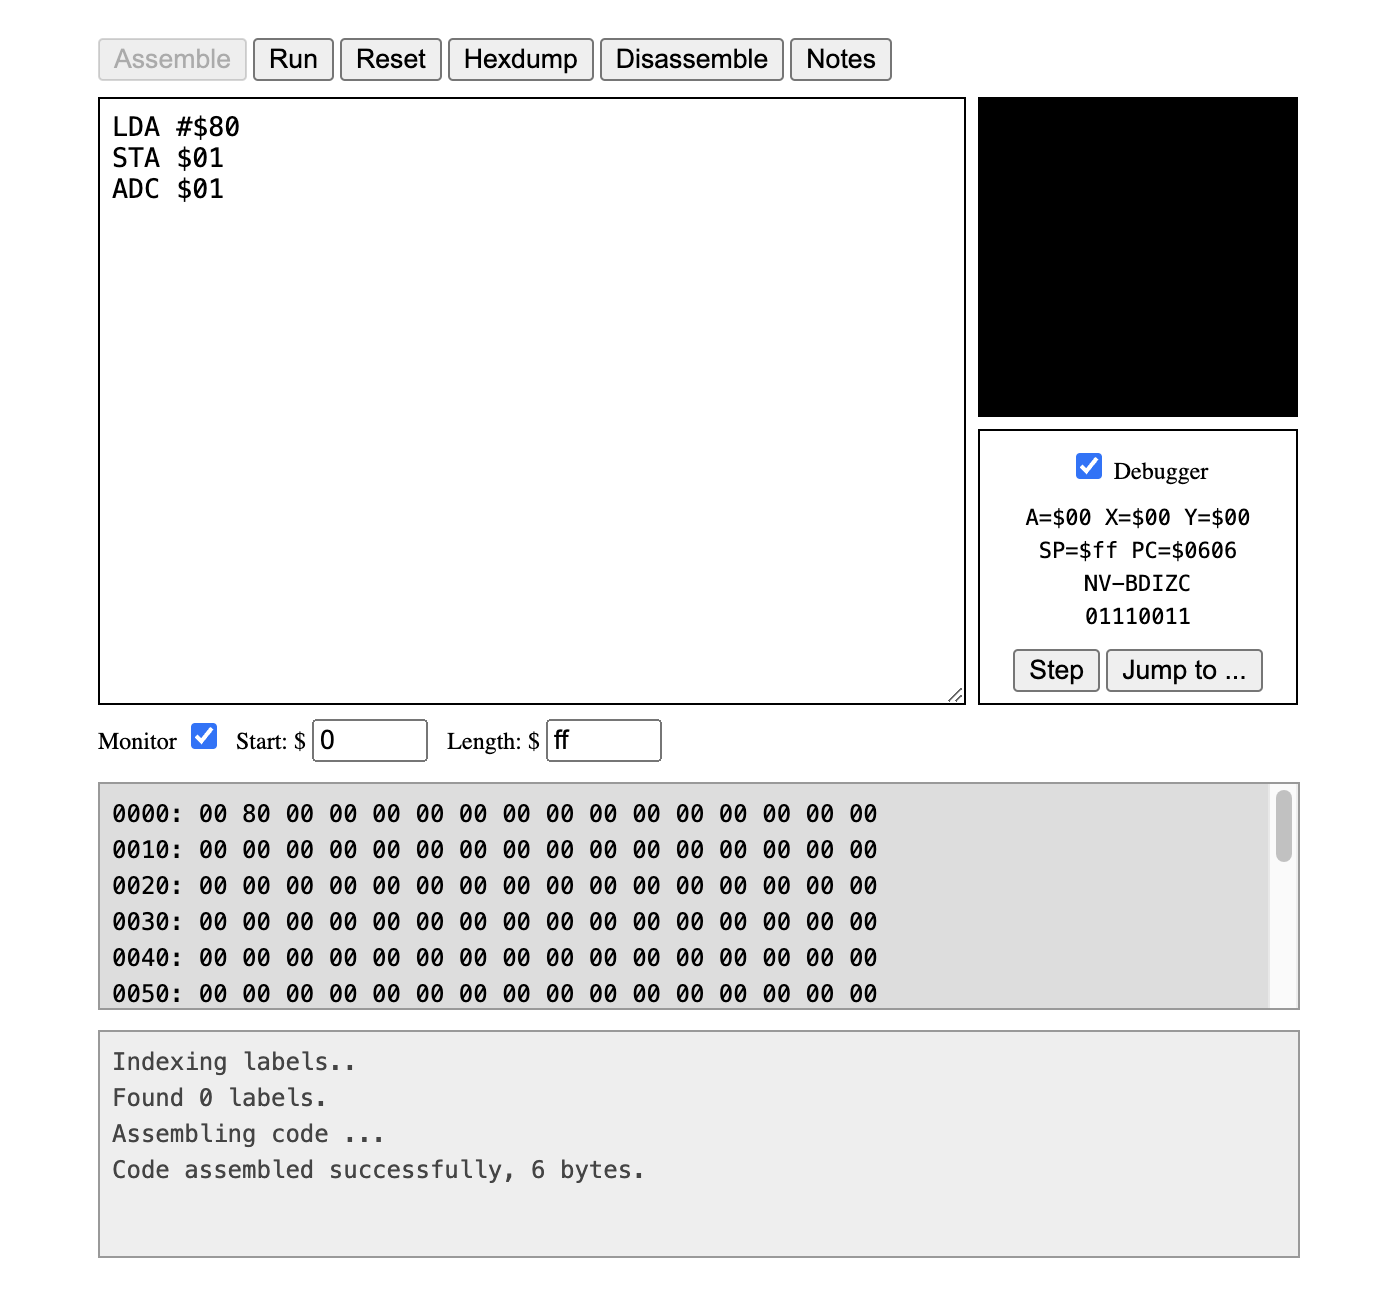
\includegraphics[width=1.0\textwidth]{res/images/q2/16-instructions-second-step3.png}
    \caption{Step 3 of second program in instructions in the 6502 simulator}
    \label{fig:16-instructions-second-step3}
\end{figure}

Finally, in \textbf{Figure \ref{fig:16-instructions-second-step3}}, the $ADC$ opcode means "ADd with Carry". And this is adding the the value at $\$01$ to the accumulator. Since $\$80 + \$80 = \$100$, the accumulator should hold $\$100$ but it doesn't because the value is bigger than a byte. Taking that into account, we can notice the things that changed in \textbf{Figure \ref{fig:16-instructions-second-step3}}. When this happens, the result is that the $A$ register is set to $\$00$ and the carry flag is set. The carry flag is the last flag in the flags byte. Another flag that has been set is the zero flag, since the result is zero.


After learning more about instructions, I will be doing the following exercises and sharing the results below:
\begin{enumerate}
    \item You've seen TAX. You can probably guess what TAY, TXA and TYA do, but write some code to test your assumptions.
    \item Rewrite the first example in this section to use the Y register instead of the X register.
    \item The opposite of ADC is SBC (subtract with carry). Write a program that uses this instruction.
\end{enumerate}

\subsubsection{Excercise 1}

I guess the meanings of the opecodes in the excercise before we start:

\begin{itemize}
    \item $TAY$: means move the value of $A$ to $Y$
    \item $TXA$: means move the value of $X$ to $A$
    \item $TYA$: means move the value of $Y$ to $A$
\end{itemize}

Here is a three pieces of code to test each one them, and I will be using the debugger to show its effect step by step.

\begin{lstlisting}[style=6502asm]
LDA #$05
TAY
\end{lstlisting}

The result of running the code to test $TAY$ is shown in \textbf{Figure \ref{fig:17-ex1-1-step1}} and in \textbf{Figure \ref{fig:18-ex1-1-step2}}.

\begin{figure}[H]
    \centering
    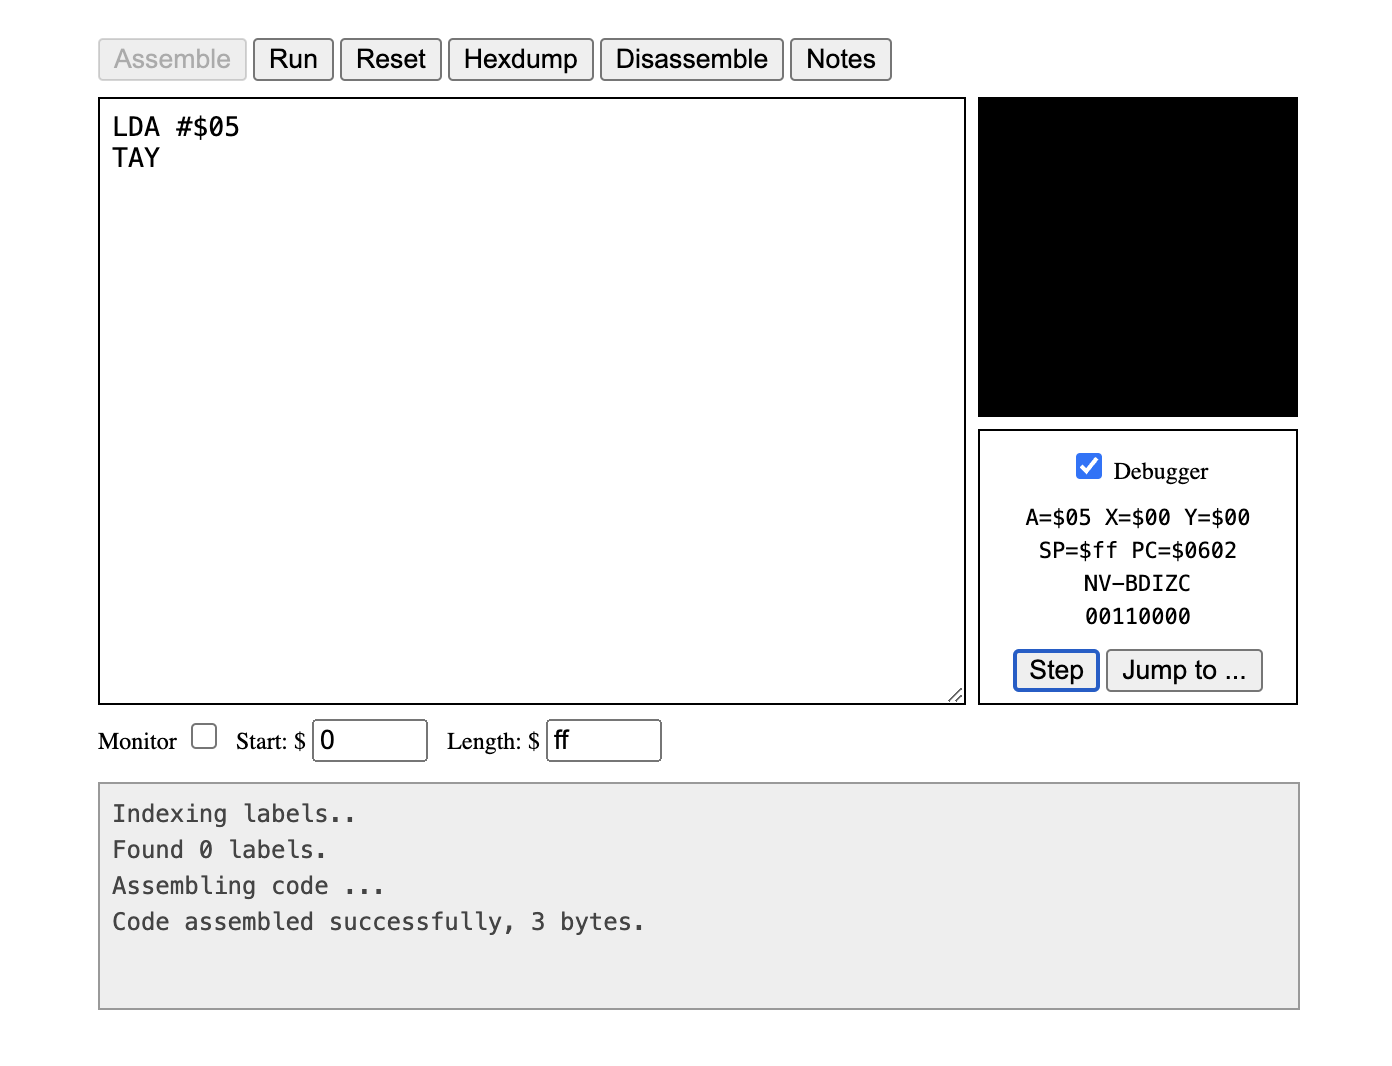
\includegraphics[width=1.0\textwidth]{res/images/q2/17-ex1-1-step1.png}
    \caption{Step 1 of first excercise program related to $TAY$ in instructions in the 6502 simulator}
    \label{fig:17-ex1-1-step1}
\end{figure}

\begin{figure}[H]
    \centering
    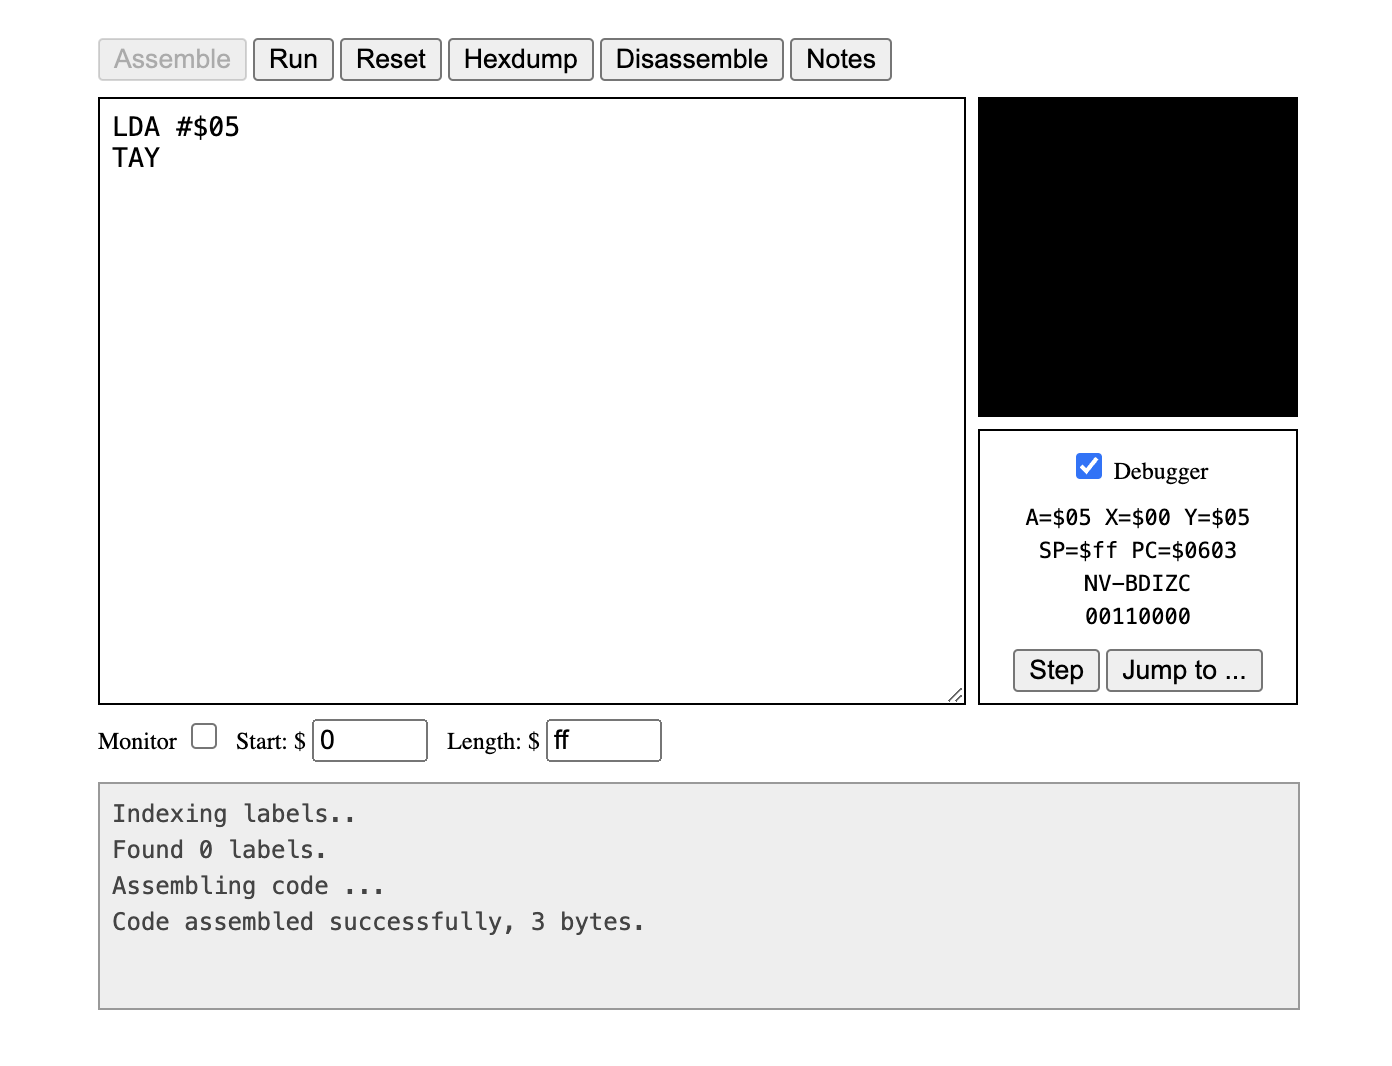
\includegraphics[width=1.0\textwidth]{res/images/q2/18-ex1-1-step2.png}
    \caption{Step 2 of first excercise program related to $TAY$ in instructions in the 6502 simulator}
    \label{fig:18-ex1-1-step2}
\end{figure}

Notice how the value of register $A$ is set in the first step in \textbf{Figure \ref{fig:17-ex1-1-step1}} and then is copied to the $Y$ register which is shown in \textbf{Figure \ref{fig:18-ex1-1-step2}}.

The two next examples will be just the steps since they can be inferred easily based on the $TAY$ explanation.

\textbf{Figure \ref{fig:19-ex1-2-step1}} and \textbf{Figure \ref{fig:20-ex1-2-step2}} show the debugger exection of $TXA$, and the code is below:


\begin{lstlisting}[style=6502asm]
LDA #$05
TAY
\end{lstlisting}

\begin{figure}[H]
    \centering
    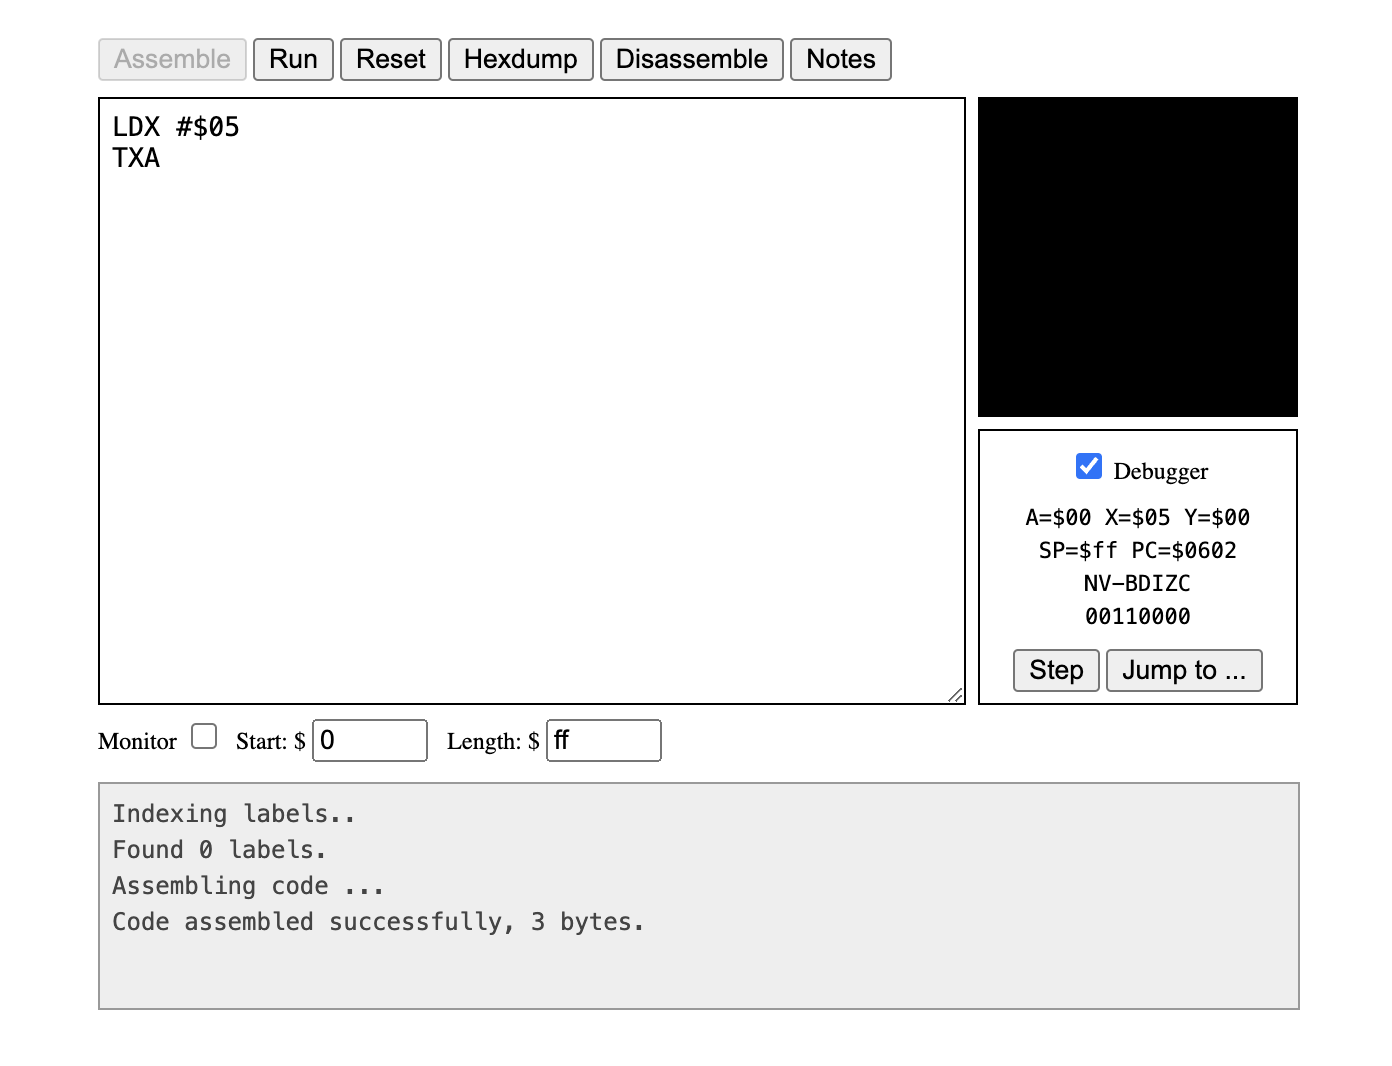
\includegraphics[width=1.0\textwidth]{res/images/q2/19-ex1-2-step1.png}
    \caption{Step 1 of first excercise program related to $TXA$ in instructions in the 6502 simulator}
    \label{fig:19-ex1-2-step1}
\end{figure}

\begin{figure}[H]
    \centering
    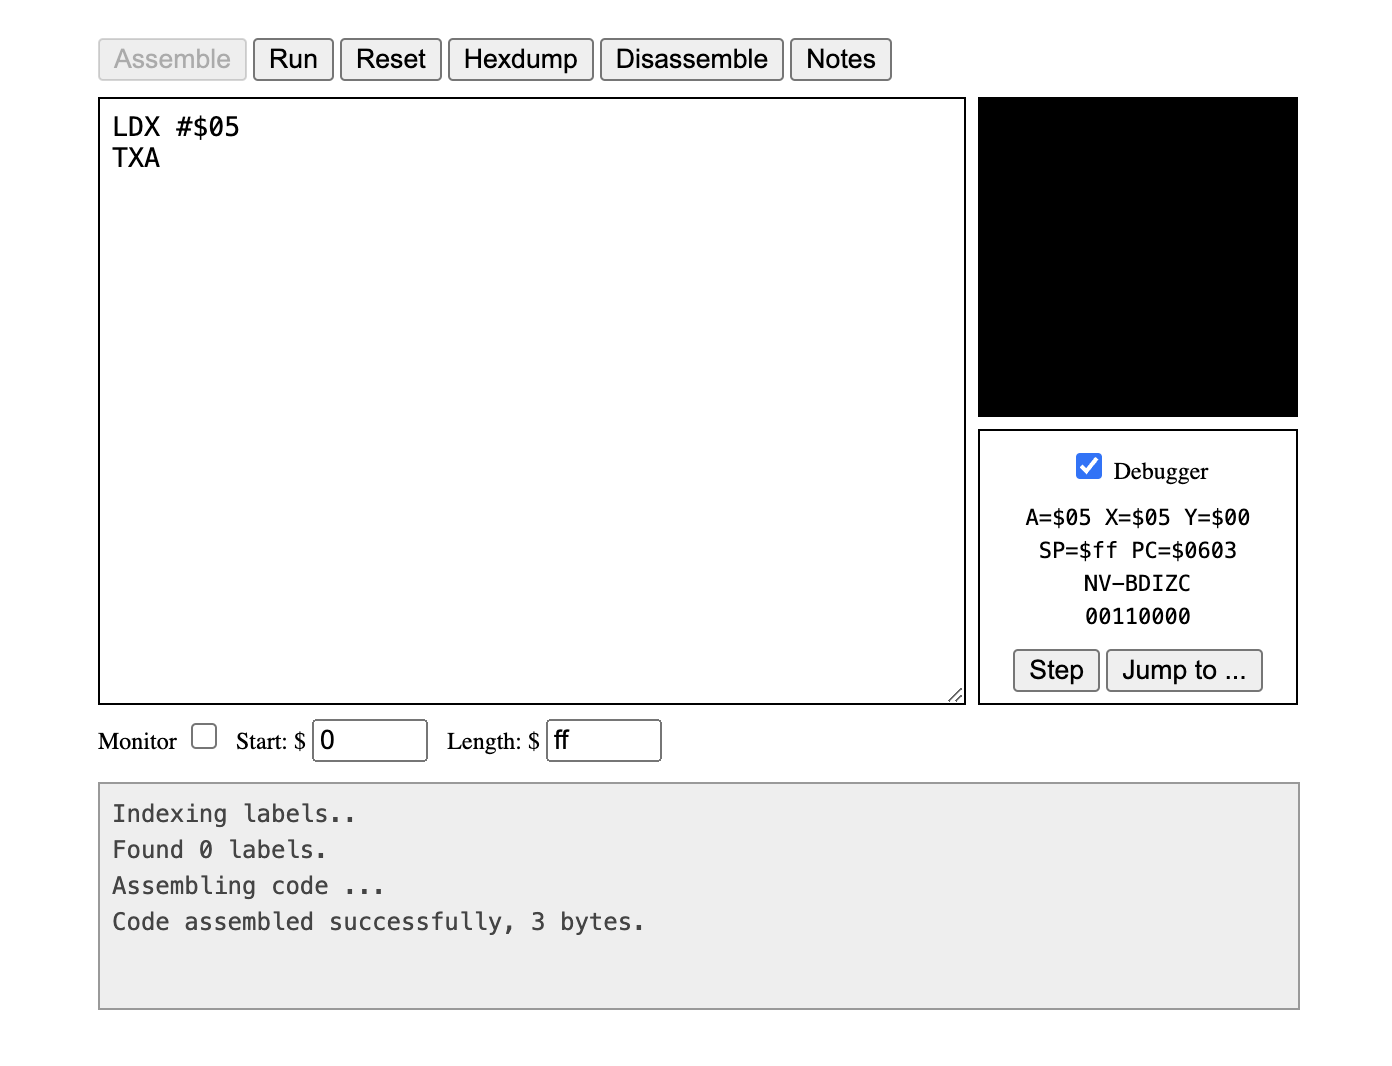
\includegraphics[width=1.0\textwidth]{res/images/q2/20-ex1-2-step2.png}
    \caption{Step 2 of first excercise program related to $TXA$ in instructions in the 6502 simulator}
    \label{fig:20-ex1-2-step2}
\end{figure}

\textbf{Figure \ref{fig:21-ex1-3-step1}} and \textbf{Figure \ref{fig:22-ex1-3-step2}} show the debugger exection of $TYA$, and the code is below:


\begin{lstlisting}[style=6502asm]
LDA #$05
TAY
\end{lstlisting}

\begin{figure}[H]
    \centering
    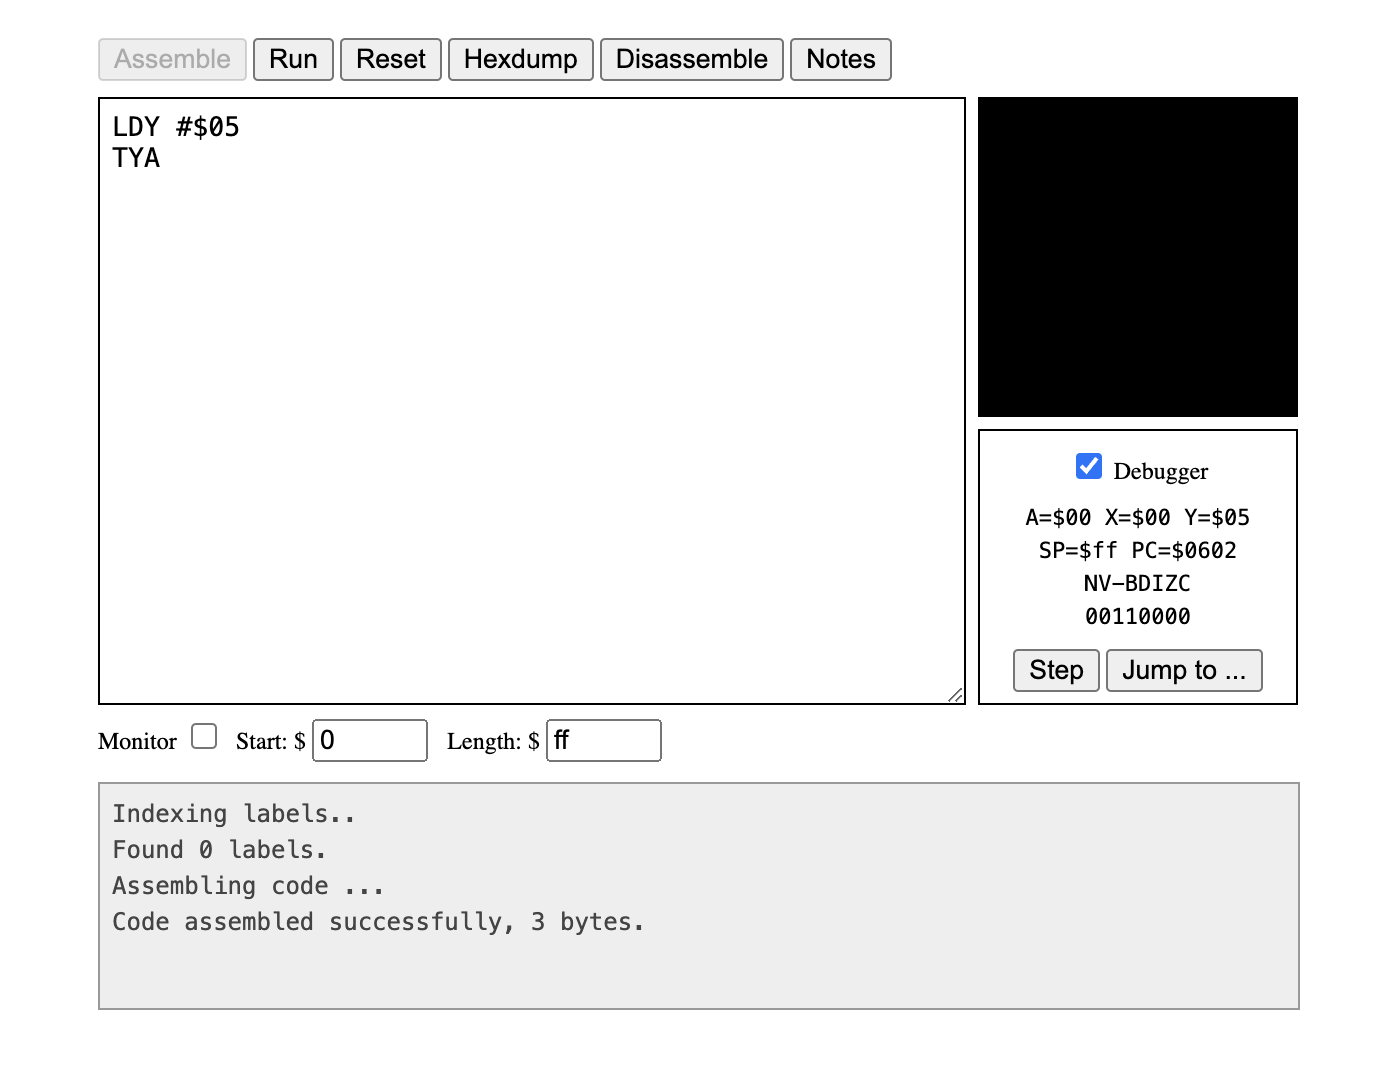
\includegraphics[width=1.0\textwidth]{res/images/q2/21-ex1-3-step1.png}
    \caption{Step 1 of first excercise program related to $TYA$ in instructions in the 6502 simulator}
    \label{fig:21-ex1-3-step1}
\end{figure}

\begin{figure}[H]
    \centering
    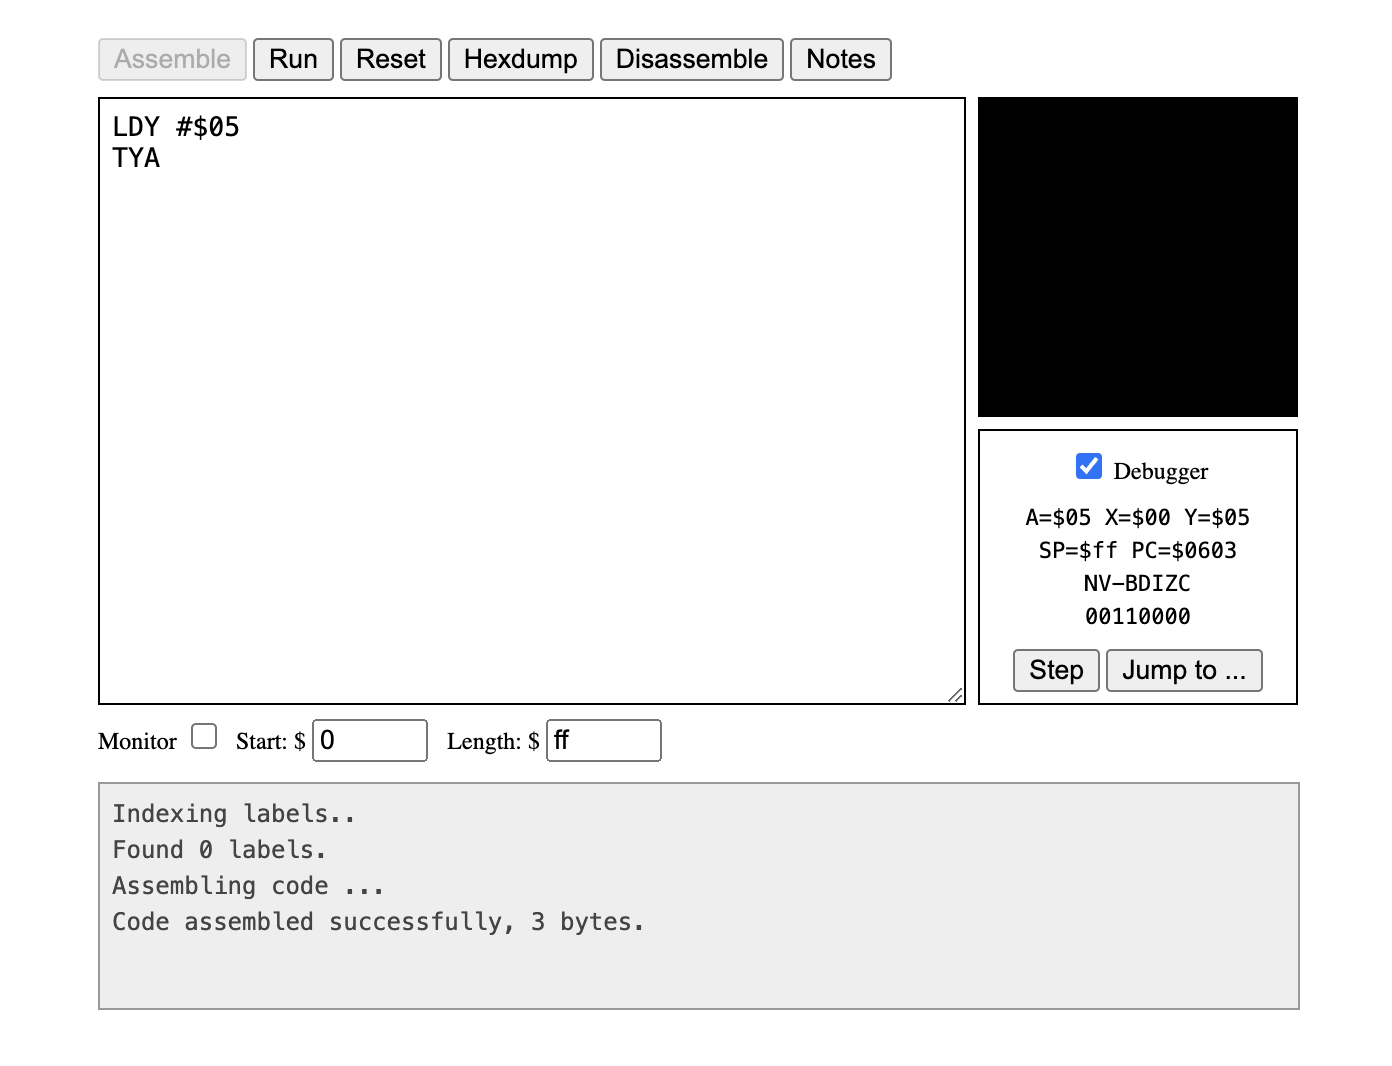
\includegraphics[width=1.0\textwidth]{res/images/q2/22-ex1-3-step2.png}
    \caption{Step 2 of first excercise program related to $TYA$ in instructions in the 6502 simulator}
    \label{fig:22-ex1-3-step2}
\end{figure}

\subsubsection{Excercise 2}

Here we will rewrite the first program in instructions section to use the $Y$ register instead of the $X$ register. Below is the new code:

\begin{lstlisting}[style=6502asm]
LDA #$c0  ;Load the hex value $c0 into the A register
TAY       ;Transfer the value in the A register to Y
INY       ;Increment the value in the Y register
ADC #$c4  ;Add the hex value $c4 to the A register
BRK       ;Break - we're done
\end{lstlisting}

And in \textbf{Figure \ref{fig:23-ex2}} we can see the result of running this code.

\begin{figure}[H]
    \centering
    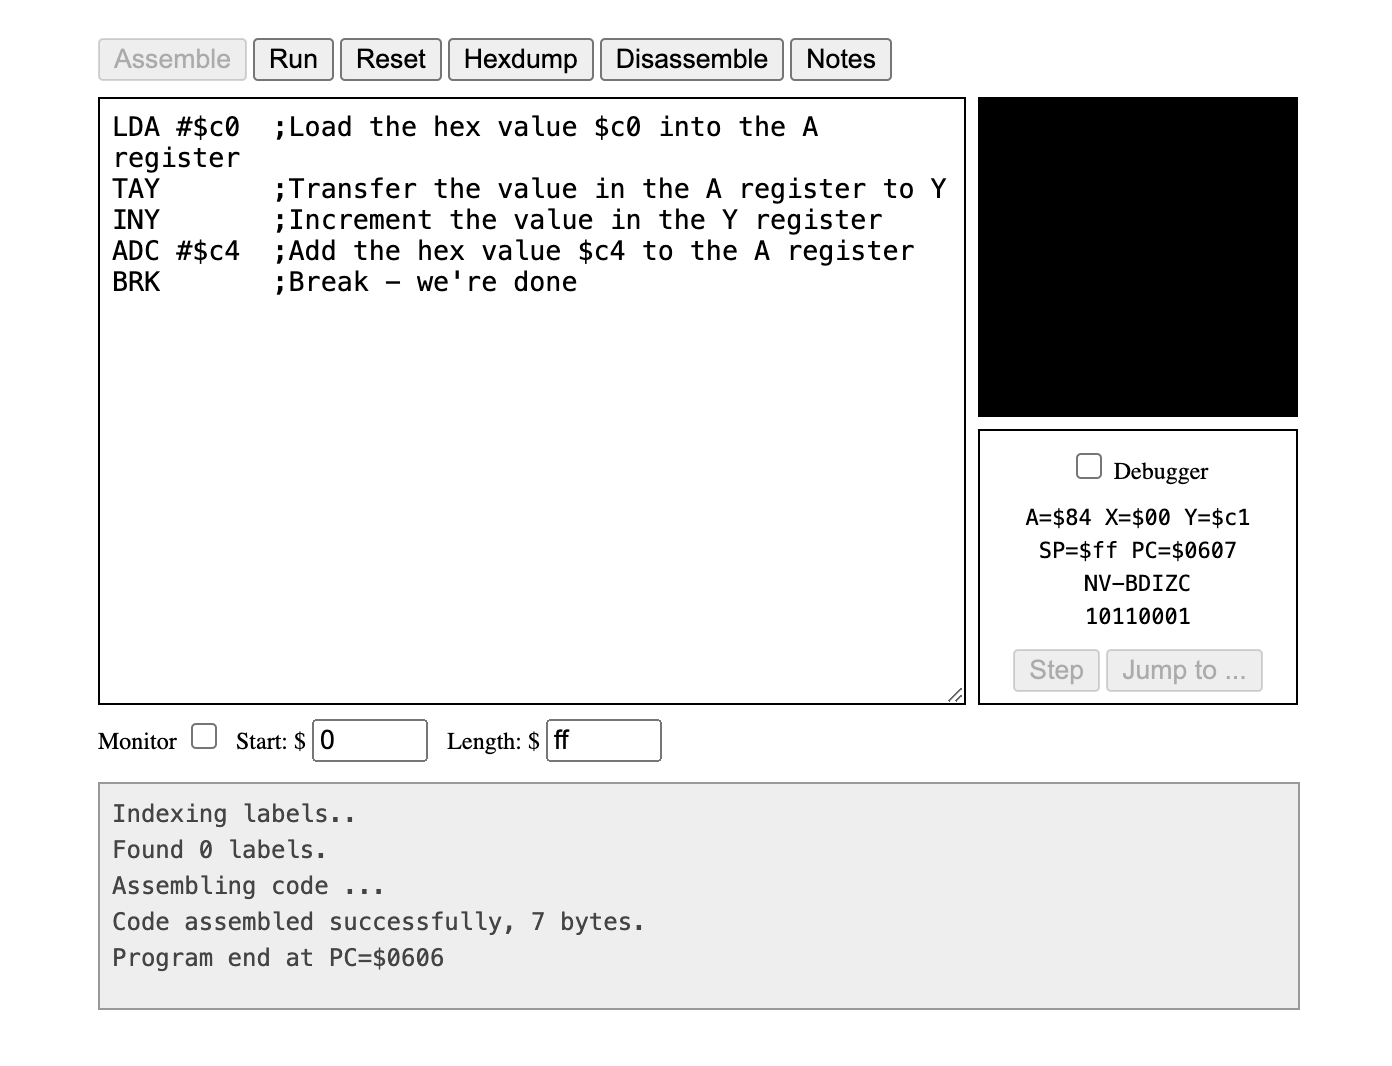
\includegraphics[width=1.0\textwidth]{res/images/q2/23-ex2.png}
    \caption{The first program but using the $Y$ istead of $X$ register in instructions in the 6502 simulator}
    \label{fig:23-ex2}
\end{figure}

\subsubsection{Excercise 3}

The code below uses $SBC$, which is (SuBtract with Carry):

\begin{lstlisting}[style=6502asm]
LDA #$ff
SBC #$0a
\end{lstlisting}

Let us step through the code using the debugger. \textbf{Figure \ref{fig:24-ex3-step1}} shows the value $\$ff$ loaded into register $A$.

\begin{figure}[H]
    \centering
    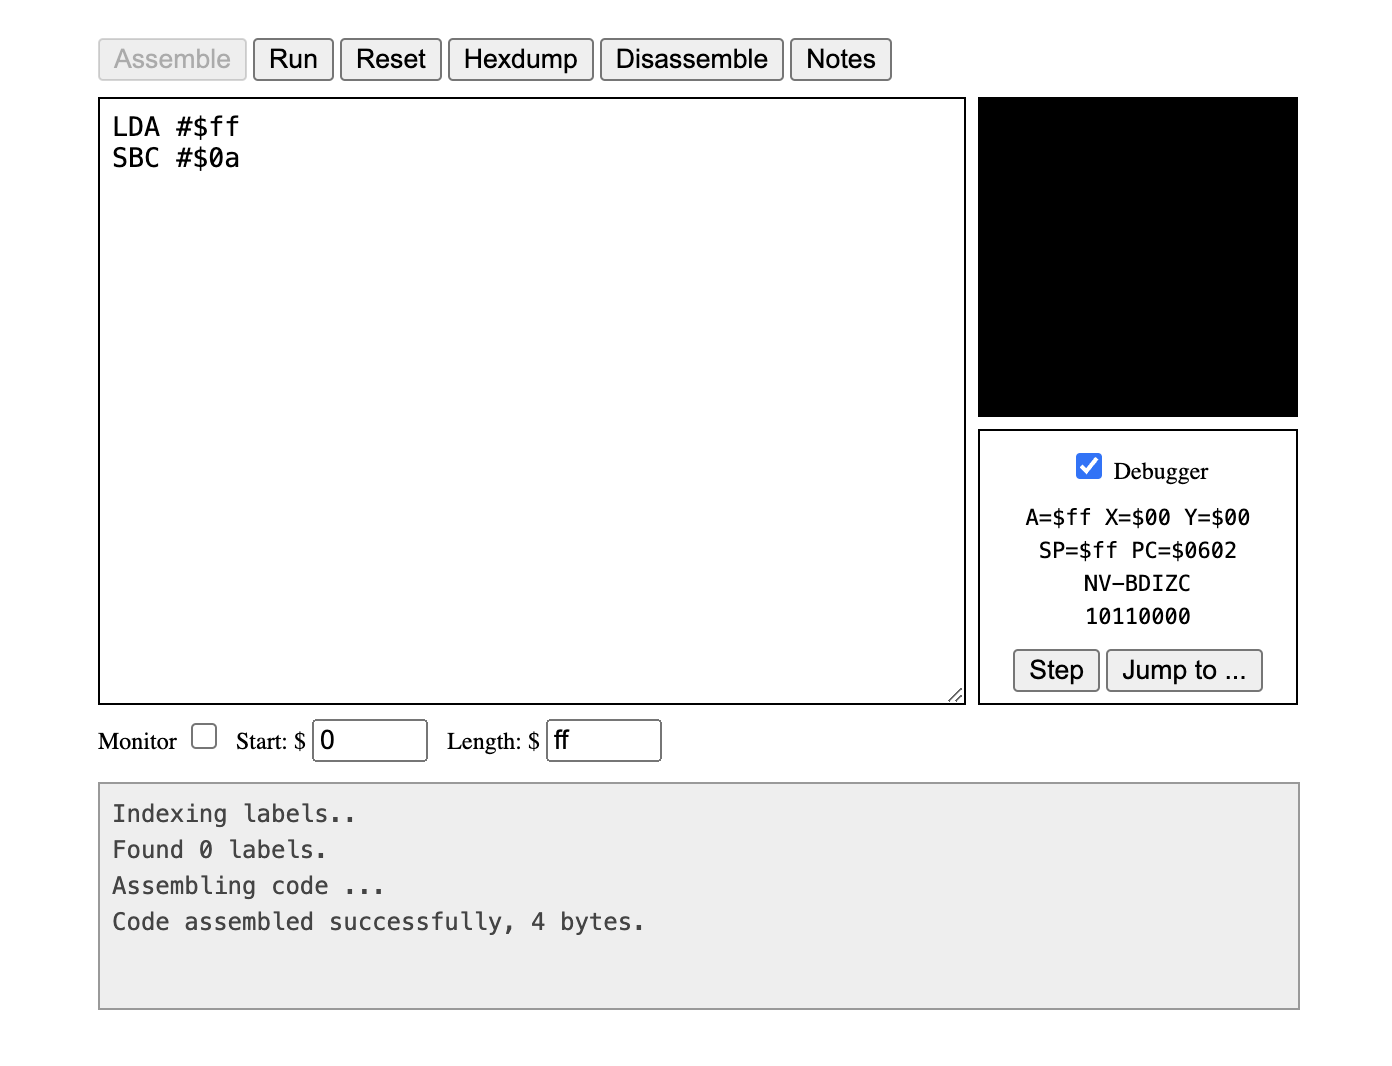
\includegraphics[width=1.0\textwidth]{res/images/q2/24-ex3-step1.png}
    \caption{The use of $SBC$ opcode in instructions in the 6502 simulator}
    \label{fig:24-ex3-step1}
\end{figure}

\end{document}